%-----------------------------------------------------------------------------%
\chapter{\babLima}
%-----------------------------------------------------------------------------%


\newcommand\MyHead[2]{%
	\multicolumn{1}{l}{\parbox{#1}{\centering #2}}
}


%-----------------------------------------------------------------------------%
\section{Implementasi}
\label{sec:implementation}
%-----------------------------------------------------------------------------%
Algoritma yang dirancang pada \autoref{sec:design} diimplementasikan dengan menggunakan beberapa bahasa pemrograman yang kemudian dikombinasikan dengan aplikasi pihak ketiga untuk menghasilkan sebuat prototipe. Subbab ini akan berisi penjabaran lengkap tentang implementasi sistem. 


%-----------------------------------------------------------------------------%
\subsection{\textit{VRP Solver}}
%-----------------------------------------------------------------------------%

\textit{VRP Solver} yang telah dirancang pada \autoref{ssec:vrp-solver} diimplementasikan dalam bahasa pemrograman C++. C++ dipilih karena memiliki manajemen \textit{resources} (\textit{processor} dan \textit{memory}) yang lebih efisien dibandingkan bahasa pemrograman lainnya, sehingga dinilai tepat untuk menangani permasalahan kombinatorial VRP yang membutuhkan komputasi yang intensif. 

\textit{Source code VRP Solver} tersedia dan dapat diunduh pada pada tautan: \url{https://github.com/soedomoto/coes-mdvrp/tree/jni-coes-mdvrp}. \textit{VRP Solver} diimplementasikan dan dikompilasi di dalam lingkungan berikut:
\begin{itemize}
	\item Sistem Operasi		: Elementary OS Loki (Berbasis Ubuntu 16.04)
	\item C++ Compiler			: c++ (Ubuntu 5.4.0-6ubuntu1~16.04.4) 5.4.0 20160609
	\item Hardware				: Asus TP300L, Quad-Core Intel® Core™ i3-4030U CPU @ 1.90GHz, 3,7 GiB DDRIII, 256GB SSD
\end{itemize}


%-----------------------------------------------------------------------------%
\subsection{\textit{Publisher} Rekomendasi}
%-----------------------------------------------------------------------------%
\textit{Publisher} rekomendasi yang tersusun atas \autoref{alg:topic-watcher} dan \autoref{alg:vrp-worker} diimplementasikan dalam bahasa pemrograman Python. Python merupakan \textit{interpreter language} dengan struktur \textit{syntax} yang simpel sehingga mudah untuk digunakan dalam penyusunan prototipe. Lingkungan yang digunakan dalam implementasi \textit{publisher} rekomendasi adalah sebagai berikut:

\begin{itemize}
	\item Sistem Operasi		: Elementary OS Loki (Berbasis Ubuntu 16.04)
	\item Python version		: Python 2.7.12
	\item Hardware				: Asus TP300L, Quad-Core Intel® Core™ i3-4030U CPU @ 1.90GHz, 3,7 GiB DDRIII, 256GB SSD
\end{itemize}

\textit{Source code} dari \textit{publisher} rekomendasi dapat diunduh di: \url{https://github.com/soedomoto/coes-mdvrp/tree/py-mdvrp-producer-redis}

%-----------------------------------------------------------------------------%
\section{Pengujian}
\label{sec:testing}
%-----------------------------------------------------------------------------%
Pengujian dilakukan untuk mengetahui tingkat ketercapaian tujuan penelitian ini yang meliputi:
\begin{itemize}
	\item Perancangan algoritma \textit{publisher} yang dapat memberikan rekomendasi terbaik secara global.
	\item Penyusunan mekanisme \textit{conflict resolution} untuk menghindari terjadinya rekomendasi lokasi yang sama pada dua atau lebih pencacah.
\end{itemize}

Akurasi algoritma diukur dengan cara membandingkan hasil pengujian sistem usulan dengan hasil pengujian algoritma MDVRP berbasis CoEAs tanpa mekanisme \textit{publish/subscribe}.


%-----------------------------------------------------------------------------%
\subsection{Lingkungan Pengujian}
\label{ssec:test-environment}
%-----------------------------------------------------------------------------%
Pengujian sistem rekomendasi lokasi dilakukan di dalam lingkungan sebagai berikut:
\begin{itemize}
	\item Sistem Operasi		: Elementary OS Loki (Berbasis Ubuntu 16.04)
	\item Redis Environment		: Redis 3.2.6, Debian Jessie (Docker version)
	\item Python version		: Python 2.7.12
	\item Hardware				: Asus TP300L, Quad-Core Intel® Core™ i3-4030U CPU @ 1.90GHz, 3,7 GiB DDRIII, 256GB SSD
\end{itemize}


%-----------------------------------------------------------------------------%
\subsection{\textit{Dataset} dan \textit{Metric}}
%-----------------------------------------------------------------------------%
%-----------------------------------------------------------------------------%
\subsubsection{\textit{Dataset}}
%-----------------------------------------------------------------------------%
Berbagai variasi data digunakan untuk memastikan validitas pengujian. Pengujian terkait \textit{Vehicle Routing Problem} umumnya dilakukan dengan memanfaatkan data Breedam, Cordeau, Solomon, Homberger, dan Russell. Data Cordeau mengandung 8 (delapan) tipe VRP \textit{problem}, sebagai berikut:

\begin{enumerate}
	\item Tipe 0 untuk kasus VRP
	\item Tipe 1 untuk kasus Periodic VRP
	\item Tipe 2 untuk kasus Multi-Depot VRP
	\item Tipe 3 untuk kasus Split Delivery VRP
	\item Tipe 4 untuk kasus VRP dengan Time Windows
	\item Tipe 5 untuk kasus Periodic VRP dengan Time Windows
	\item Tipe 6 untuk kasus Multi-Depot VRP dengan Time Windows
	\item Tipe 7 untuk kasus Split Delivery VRP dengan Time Windows
\end{enumerate}

Pada penelitian ini, pengujian dilakukan dengan menggunakan dataset Cordeau tipe 2 (Multi-Depot VRP), dengan struktur format sebagai berikut:
\begin{enumerate}
	\item Baris pertama berformat \textbf{TYPE M N T}, dimana: \\
	M = Jumlah \textit{vehicle} \\
	N = Jumlah \textit{customer} \\
	T = Jumlah \textit{depot}
	
	\item Baris kedua sampai T baris berikutnya berformat \textbf{D Q}, dimana: \\
	D = Durasi maksimum dari setiap rute \\
	Q = Kapasitas maksumum dari setiap \textit{vehicle}
	
	\item Baris selanjutnya sampai M baris berikutnya berformat \textbf{i x y d q f a list e l}, dimana: \\
	i	= nomer \textit{customer} \\
	x	= koordinat x \\
	y	= koordinat y \\
	d	= durasi pelayanan (\textit{service time}) \\
	q	= \textit{demand} \\
	f	= frekuensi kunjungan \\
	a	= jumlah kombinasi kunjungan \\
	list	= list dari semua kombinasi kunjungan \\
	e	= jika ada, waktu dimulainya kunjungan \\
	l	= jika ada, waktu selesainya kunjungan
	
	\item Baris selanjutnya sampai M baris berikutnya berformat \textbf{i x y}, dimana: \\
	i	= nomer \textit{vehicle} \\
	x	= koordinat depot x \\
	y	= koordinat depot y \\
\end{enumerate}

Untuk menyimulasikan kondisi lapangan yang sebenarnya, sistem juga diuji dengan menggunakan data lapangan wilayah administratif di Kabupaten Pesisir Selatan, Provinsi Sumatera Barat. Data lapangan merepresentasikan kondisi pencacahan yang sebenarnya, dimana terdapat \textit{cost} berupa jarak dan waktu tempuh antar lokasi (\textit{node}). 

Data lapangan yang digunakan meliputi:
\begin{itemize}
	\item data 182 lokasi pencacahan beserta posisi koordinatnya yang dianalogikan sebagai \textit{customer} (N = 182). 
	\item data 15 petugas pencacahan yang dianalogikan sebagai \textit{vehicle} ($M$ = 15) beserta koordinat \textit{initial depot} tiap-tiap pencacah.
\end{itemize}

Untuk setiap kombinasi lokasi pencacahan dan \textit{initial depot} dari petugas, dilakukan penghitungan waktu tempuhnya dengan memanfaatkan \textit{Google Direction API}, sebagaimana dijelaskan pada \autoref{ss:distance-duration-matrix}.


%-----------------------------------------------------------------------------%
\subsubsection{\textit{Metric}}
\label{sssec:metric}
%-----------------------------------------------------------------------------%
Sistem usulan yang menggunakan algoritma MDVRP berbasis CoEAs dan mekanisme \textit{publish/subscribe} akan dibandingkan dengan program pembanding yang menggunakan algoritma yang sama, namun tanpa mekanisme \textit{publish/subscribe}. Masing-masing pengujian akan menghasilkan output berupa rute untuk setiap petugas pencacahan seperti contoh berikut:

\begin{itemize}
	\item \textit{Vehicle} A = Loc1 $\rightarrow$ Loc5 $\rightarrow$ Loc15 $\rightarrow$ Loc12
	\item \textit{Vehicle} B = Loc 6 $\rightarrow$ Loc2 $\rightarrow$ Loc16 $\rightarrow$ Loc3
	\item \textit{Vehicle} C = Loc4 $\rightarrow$ Loc8 $\rightarrow$ Loc14 $\rightarrow$ Loc 7
	\item \textit{Vehicle} D = Loc9 $\rightarrow$ Loc10 $\rightarrow$ Loc11 $\rightarrow$ Loc12
\end{itemize}


\begin{figure}[!]
	\centering
	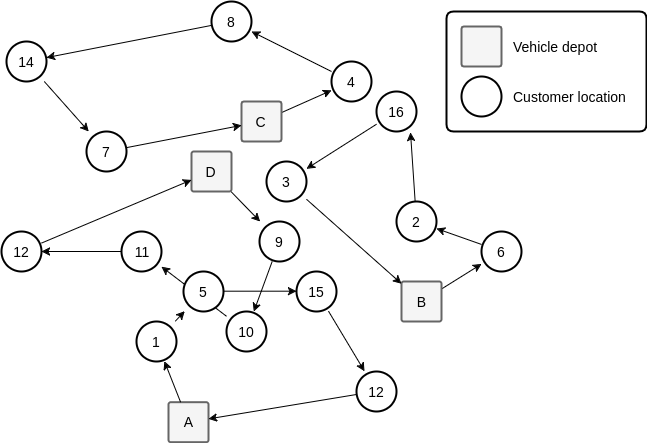
\includegraphics[width=9cm]{Resources/Images/result-mdvrp-illustration}
	\caption{Ilustrasi Rute yang Dihasilkan}
	\label{fig:result-mdvrp-illustration}
\end{figure}


Biaya total untuk tiap-tiap rute kemudian dihitung dengan melakukan penjumlahan seluruh waktu tempuh dan waktu pelayanan (\textit{service time}) dari lokasi yang dikunjungi. Pada contoh \autoref{fig:result-mdvrp-illustration}, biaya total dari setiap kendaraan adalah:

\begin{itemize}
	\item $TC_A$ = $C_{A-1}$ + $ST_5$ + $C_{1-5}$ + $ST_5$ + $C_{5-15}$ + $ST_15$ + $C_{15-12}$ + $ST_12$ + $C_{12-A}$
	\item $TC_B$ = $C_{B-6}$ + $ST_6$ + $C_{6-2}$ + $ST_2$ + $C_{2-16}$ + $ST_16$ + $C_{16-3}$ + $ST_3$ + $C_{3-B}$
	\item $TC_C$ = $C_{C-4}$ + $ST_4$ + $C_{4-8}$ + $ST_8$ + $C_{8-14}$ + $ST_14$ + $C_{14-7}$ + $ST_7$ + $C_{7-C}$
	\item $TC_D$ = $C_{D-9}$ + $ST_9$ + $C_{9-10}$ + $ST_10$ + $C_{10-11}$ + $ST_11$ + $C_{11-12}$ + $ST_12$ + $C_{12-D}$
\end{itemize}
dimana TC adalah \textit{total cost}, C adalah \textit{transport cost} yang merupakan waktu tempuh, dan ST adalah \textit{service time}. Seluruh biaya direpresentasikan dalam satuan waktu.


Setelah waktu total dari tiap-tiap rute diperoleh, kemudian waktu total untuk keseluruhan rute dan standar deviasi waktu total dari keseluruhan rute dapat dikalkulasi. \textbf{\textit{Metric}} yang digunakan untuk mengukur perbandingan antar pengujian adalah standar deviasi waktu total dari seluruh rute yang dihasilkan oleh sistem usulan maupun sistem pembanding. Standar deviasi dipilih sebagai \textit{metric} karena lebih merepresentasikan kondisi pencacahan yang sebenarnya, dimana semakin kecil variasi waktu antar petugas, semakin merata beban tugas yang berimbas pada waktu penyelesaian pencacahan secara keseluruhan akan lebih cepat. Sistem yang lebih baik akan menghasilkan standar deviasi yang lebih kecil.


%-----------------------------------------------------------------------------%
\subsection{Skenario dan Hasil Pengujian}
%-----------------------------------------------------------------------------%
Pengujian dilakukan dengan beberapa skenario untuk memastikan bahwa program dapat bekerja dengan baik pada kondisi yang berbeda-beda. Skenario yang digunakan dalam pengujian dan hasilnya akan dijabarkan secara lebih detail pada \autoref{sssec:test-no-service-time} hingga \autoref{sssec:test-delay-service-time}.


Komponen yang terlibat dalam pengujian terdiri dari pencacah, \textit{message broker}, \textit{publisher} rekomendasi, \textit{vrp solver}, dan \textit{shared memory}. \textit{Setup} dari tiap-tiap komponen dijelaskan pada \autoref{ssec:broker-setup} sampai \autoref{sssec:subscriber-setup}. Interaksi yang terjadi antar komponen, seperti digambarkan \autoref{fig:component-interaction}, adalah sebagai berikut:


\begin{enumerate}
	\item Pencacah melakukan \textit{subscription} dengan menggunakan 'lokasi terkini' sebagai topik.
	\item Publisher (\textit{topic watcher}) memantau setiap topik yang di-\textit{subscribe}.
	\item VRP Solver melakukan kalkulasi rute untuk mendapatkan rute terbaik.
	\item Rute yang diperoleh dikembalikan ke \textit{publisher} untuk dipilah menurut topiknya.
	\item \textit{Publisher} mem-\textit{publish} rute kepada pencacah yang melakukan \textit{subscription} melalui \textit{message broker}.
	\item Pesan dari \textit{publisher} diteruskan kepada pencacah sesuai dengan topiknya.
	\item Pada saat pencacah sampai pada lokasi pencacahan, maka lokasi terkini dari setiap pencacah disimpan ke \textit{shared memory}.
	\item \textit{Shared memory} yang tersimpan akan digunakan oleh publisher dalam mendefinisikan masalah yang akan diselesaikan, yang terdiri dari definisi pencacah, lokasi pencacahan, dan jarak antar lokasi.
\end{enumerate}


\begin{figure}[!]
	\centering
	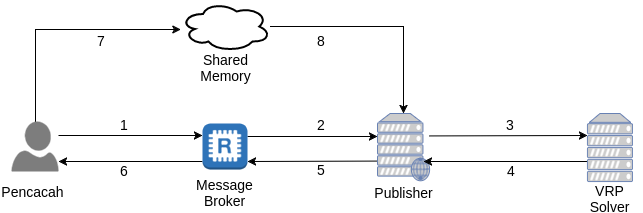
\includegraphics[width=\textwidth]{Resources/Images/component-interaction}
	\caption{Interaksi antar komponen dalam pengujian}
	\label{fig:component-interaction}
\end{figure}


%-----------------------------------------------------------------------------%
\subsubsection{\textit{Message Broker Setup}}
\label{ssec:broker-setup}
%-----------------------------------------------------------------------------%
Seluruh skenario dalam pengujian ini akan menggunakan Redis sebagai \textit{message broker}. Redis merupakan \textit{in-memory data structure store} yang dapat digunakan sebagai \textit{database}, \textit{cache}, dan \textit{message broker} \citep{redis_introduction_2017}. Redis mempunyai \textit{feature} Redis Cluster, sehingga dapat dengan mudah disusun menjadi \textit{distributed message broker}. Selain itu, Redis \textit{client} tersedia dalam sebagian besar bahasa pemrograman \citep{redis_clients_2017}, sehingga memungkinkan pemilihan bahasa pemrograman dalam implementasi sistem secara lebih fleksibel.


Pada penelitian ini, Redis Cluster dikonfigurasi dengan menggunakan 6 (enam) buah \textit{nodes}, 3 (tiga) node digunakan sebagai \textit{master} dan sisanya sebagai \textit{slave}. Konfigurasi Redis Cluster pada setiap node diilustrasikan pada Kode \autoref{lst:redis_conf}. Dalam konteks Redis, master dapat dianggap sebagai partisi, dan slave dianggap sebagai replikasi dari master. Seluruh node, baik master maupun slave dapat digunakan sebagai \textit{entrypoint} dimana client terkoneksi.


\begin{listing}[!]
	\caption{Konfigurasi Redis Cluster}
	\label{lst:redis_conf}
	\begin{minted}[showspaces=false,breaklines=true]{java}
cluster-enabled yes
cluster-node-timeout 5000
cluster-config-file nodes.conf
appendonly yes
dir /data
	\end{minted}
\end{listing}


\textit{Nodes} Redis yang telah dikonfigurasi dan dijalankan, dapat digunakan untuk membuat cluster dengan memanfaatkan  \textit{script} \textbf{redis-trib.rb} yang telah disediakan oleh Redis. \textit{Command} yang digunakan dalam pembuatan cluster serta  \textit{response} yang diperoleh diilustrasikan pada Kode \autoref{lst:redis_trib_cluster} dan \autoref{lst:redis_trib_cluster_response}. \autoref{fig:test-flowchart-normal-global-broker} 
menyajikan \textit{flowchart} subsistem \textit{message broker setup}. 


\begin{listing}[!]
	\caption{Pembuatan Redis Cluster}
	\label{lst:redis_trib_cluster}
	\begin{minted}[showspaces=false,breaklines=true]{java}
/redis-trib.rb create --replicas 1 172.17.0.3 172.17.0.4 172.17.0.5 172.17.0.6 172.17.0.7 172.17.0.8
	\end{minted}
\end{listing}


\begin{listing}[!]
	\caption{Respon Pembuatan Redis Cluster}
	\label{lst:redis_trib_cluster_response}
	\begin{minted}[showspaces=false,breaklines=true]{java}
Creating cluster
Performing hash slots allocation on 6 nodes...
Using 3 masters:
172.17.0.3:6379
172.17.0.4:6379
172.17.0.5:6379
Adding replica 172.17.0.6:6379 to 172.17.0.3:6379
Adding replica 172.17.0.7:6379 to 172.17.0.4:6379
Adding replica 172.17.0.8:6379 to 172.17.0.5:6379
M: 2f0c681921fe52900a6774fb2cc808a8c4e69216 172.17.0.3:6379
slots:0-5460 (5461 slots) master
M: 41a343142847138301ceeb710206284a50bb44a0 172.17.0.4:6379
slots:5461-10922 (5462 slots) master
M: 88ae20b9e75dd5aa58973f13aa89479f52cedfd3 172.17.0.5:6379
slots:10923-16383 (5461 slots) master
S: c5f6764d82ed10793c0c81e54830b4f68b1eacd7 172.17.0.6:6379
replicates 2f0c681921fe52900a6774fb2cc808a8c4e69216
S: 5906f61963d4a5a45478736d976b79db4280b3c7 172.17.0.7:6379
replicates 41a343142847138301ceeb710206284a50bb44a0
S: 635ed817b134b5d14bffd61fe9089867037fee8c 172.17.0.8:6379
replicates 88ae20b9e75dd5aa58973f13aa89479f52cedfd3
Can I set the above configuration? (type 'yes' to accept): yes
Nodes configuration updated
Assign a different config epoch to each node
Sending CLUSTER MEET messages to join the cluster
Waiting for the cluster to join...
Performing Cluster Check (using node 172.17.0.3:6379)
M: 2f0c681921fe52900a6774fb2cc808a8c4e69216 172.17.0.3:6379
slots:0-5460 (5461 slots) master
1 additional replica(s)
M: 88ae20b9e75dd5aa58973f13aa89479f52cedfd3 172.17.0.5:6379
slots:10923-16383 (5461 slots) master
1 additional replica(s)
S: c5f6764d82ed10793c0c81e54830b4f68b1eacd7 172.17.0.6:6379
slots: (0 slots) slave
replicates 2f0c681921fe52900a6774fb2cc808a8c4e69216
M: 41a343142847138301ceeb710206284a50bb44a0 172.17.0.4:6379
slots:5461-10922 (5462 slots) master
1 additional replica(s)
S: 635ed817b134b5d14bffd61fe9089867037fee8c 172.17.0.8:6379
slots: (0 slots) slave
replicates 88ae20b9e75dd5aa58973f13aa89479f52cedfd3
S: 5906f61963d4a5a45478736d976b79db4280b3c7 172.17.0.7:6379
slots: (0 slots) slave
replicates 41a343142847138301ceeb710206284a50bb44a0
[OK] All nodes agree about slots configuration.
Check for open slots...
Check slots coverage...
[OK] All 16384 slots covered.
	\end{minted}
\end{listing}


%-----------------------------------------------------------------------------%
\subsubsection{\textit{Publisher Setup}}
%-----------------------------------------------------------------------------%
Publisher dikonfigurasi dan dijalankan pada lingkungan yang telah didefinisikan pada \autoref{ssec:test-environment}, sesuai dengan alur yang digambarkan pada \autoref{fig:test-flowchart-normal-global-publisher}. Format penggunaan Publisher diilustrasikan pada \autoref{lst:publisher-usage}.


\begin{listing}[!]
	\caption{Format penggunaan Publisher}
	\label{lst:publisher-usage}
	\begin{minted}[showspaces=false,breaklines=true]{bash}
Usage: mdvrp-redis-producer [options]

Run location recommendation server

Options:
-h, --help            show this help message and exit
-b BIN, --coes-bin=BIN
Binary of CoES MDVRP library
-D D, --data=D        Data problem file
-C C, --cost-file=C   Cost matrix file
-O O, --output-dir=O  Output directory
-t, --use-timestamp   Append timestamp to output directory
-B B, --broker-url=B  Redis broker URL
-X X, --solver-execution-time=X
VRP Solver execution time
	\end{minted}
\end{listing}


%-----------------------------------------------------------------------------%
\subsubsection{\textit{Subscriber Setup}}
\label{sssec:subscriber-setup}
%-----------------------------------------------------------------------------%
Pengujian memerlukan sebuah program tambahan yang berperan sebagai pencacah/\textit{subscriber}. Alur kerja dari tiap-tiap \textit{subscriber} (\autoref{fig:test-flowchart-normal-global-subscriber}) adalah sebagai berikut:


\begin{enumerate}
	\item Lakukan \textit{subscription} (pengiriman \textit{request}) pada \textit{message broker} dengan topik \textit{current location} dari \textit{subscriber}. 
	\item Sebuat \textit{reply} akan diterima dari \textit{publisher} yang dikirim melalui \textit{message broker} berupa lokasi pencacahan berikutnya yang akan dikunjungi. 
	\item Lakukan perjalanan ke lokasi yang akan dikunjungi yang disimulasikan dengan `\textit{sleep}'
	\item Setelah tiba di lokasi, simpan \textit{current location} pada \textit{shared memory} 
	\item Lakukan pencacahan yang disimulasikan dengan \textit{sleep}, 
	\item Ulangi proses dari langkah pertama.
\end{enumerate}


\begin{figure}[!]
	\centering
	\begin{subfigure}[t]{0.3\textwidth}
		\centering
		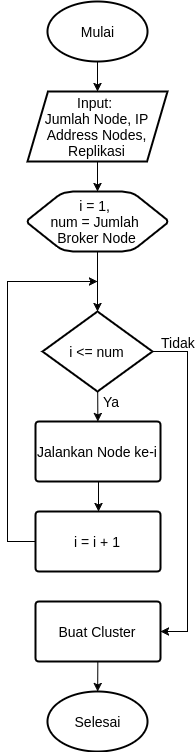
\includegraphics[width=\textwidth]{Resources/Images/test-flowchart-normal-global-broker}
		\caption{\textit{Flowchart Message Broker}}
		\label{fig:test-flowchart-normal-global-broker}
	\end{subfigure}%
	~
	\begin{subfigure}[t]{0.39\textwidth}
		\centering
		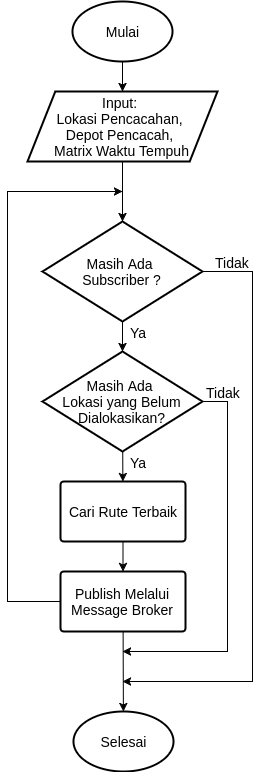
\includegraphics[width=\textwidth]{Resources/Images/test-flowchart-normal-global-publisher}
		\caption{\textit{Flowchart Publisher}}
		\label{fig:test-flowchart-normal-global-publisher}
	\end{subfigure}%
	~
	\begin{subfigure}[t]{0.31\textwidth}
		\centering
		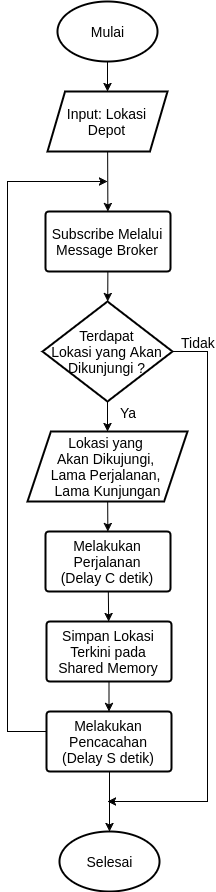
\includegraphics[width=\textwidth]{Resources/Images/test-flowchart-normal-global-subscriber}
		\caption{\textit{Flowchart Subscriber}}
		\label{fig:test-flowchart-normal-global-subscriber}
	\end{subfigure}
	\caption{\textit{Flowchart} Subsistem pada Pengujian}
	\label{fig:test-flowchart-normal-global}
\end{figure}


%-----------------------------------------------------------------------------%
\subsubsection{Pengujian Tanpa \textit{Service Time}}
\label{sssec:test-no-service-time}
%-----------------------------------------------------------------------------%
Pengujian ini bertujuan membandingkan keakuratan sistem dalam memproses data tanpa melibatkan \textit{service time} dari \textit{customer}-nya. Data \textit{subscriber} dan \textit{customer} di-\textit{generate} secara random, baik dalam hal jumlah maupun koordinat lokasi. Data yang digunakan diperoleh dari \textit{instance} Cordeau P01 sampai P10, dengan tiap-tiap komposisi sebagai berikut:


\begin{enumerate}
	\item Instance P01 terdiri dari 50 \textit{customer} dan 5 \textit{vehicle},
	\item Instance P02 terdiri dari 50 \textit{customer} dan 4 \textit{vehicle}, 
	\item Instance P03 terdiri dari 75 \textit{customer} dan 5 \textit{vehicle}, 
	\item Instance P04 terdiri dari 100 \textit{customer} dan 2 \textit{vehicle}, 
	\item Instance P05 terdiri dari 100 \textit{customer} dan 2 \textit{vehicle}, 
	\item Instance P06 terdiri dari 100 \textit{customer} dan 3 \textit{vehicle}, 
	\item Instance P07 terdiri dari 100 \textit{customer} dan 4 \textit{vehicle}, 
	\item Instance P08 terdiri dari 249 \textit{customer} dan 2 \textit{vehicle}, 
	\item Instance P09 terdiri dari 249 \textit{customer} dan 3 \textit{vehicle}, 
	\item Instance P10 terdiri dari 249 \textit{customer} dan 4 \textit{vehicle}.
\end{enumerate}
Terminologi \textit{vehicle} dan \textit{customer} pada data Cordeau analog dengan pencacah dan lokasi pencacahan pada permasalahan rekomendasi lokasi pencacahan.


Setiap \textit{instance} data diuji sebanyak 5 (lima) kali untuk membuktikan bahwa hasil yang diperoleh konsisten. Dari hasil simulasi, diperoleh rute untuk tiap-tiap \textit{instance} sebagaimana digambarkan pada \hyperref[ch:test_result_cordeau_notw]{Lampiran 1}. Berdasarkan rute-rute ini kemudian dilakukan penghitungan untuk:
\begin{enumerate}
	\item Waktu total untuk setiap rute.
	\item Waktu total untuk seluruh rute yang ada pada setiap \textit{instance} (\autoref{tbl:test_result_p01_notw_total_time} - \autoref{tbl:test_result_p10_notw_total_time}).
	\item Rata-rata total waktu seluruh rute dari 5 kali pengujian untuk setiap \textit{instance} \autoref{tbl:test_result_cordeau_notw_total_time}.
	\item Standar deviasi dari total waktu seluruh rute, sesuai dengan cara yang dijelaskan pada \autoref{sssec:metric}. Hasil penghitungan standar deviasi dari seluruh rute pada setiap \textit{instance} disajikan pada \autoref{tbl:test_result_p01_notw_standard_deviation_of_total_time} - \autoref{tbl:test_result_p10_notw_standard_deviation_of_total_time}. Untuk setiap \textit{instance}, kemudian dihitung rata-rata standar deviasi terhadap 5 (lima) pengujian yang telah dilakukan.
\end{enumerate}


Hasil pengujian, seperti digambarkan pada \autoref{fig:test_result_10_cordeau_total_time} menunjukkan bahwa sistem pembanding (CoEAs + MDVRP) lebih unggul dari \textbf{segi total waktu pencacahan (penjumlahan total waktu dari seluruh rute)}, dimana 9 dari 10 \textit{instance} yang diujikan memiliki total waktu yang lebih kecil jika diproses dengan sistem pembanding, seperti dirincikan pada \autoref{tbl:test_result_cordeau_notw_total_time}. Namun, dari segi \textbf{standar deviasi total waktu dari seluruh rute} seperti digambarkan pada \autoref{fig:test_result_10_cordeau_standard_deviation}, sistem usulan (CoEAs + MDVRP + \textit{publish/subscribe}) lebih unggul, dimana 8 dari 10 \textit{instance} yang diujikan dengan sistem usulan menghasilkan standar deviasi yang lebih kecil dibandingkan standar deviasi dari sistem pembanding, seperti dirincikan pada \autoref{tbl:test_result_cordeau_notw_standard_deviation_of_total_time}. Hal ini memperkuat kesimpulan bahwa sistem usulan memberikan rekomendasi rute yang lebih baik dibandingkan sistem pembanding. 


Standar deviasi yang kecil berarti terdapat waktu penyelesaian tugas antar pencacah yang hampir setara, sehingga seluruh kegiatan pencacahan dapat selesai pada waktu yang hampir bersamaan. Hal ini berbanding terbalik dengan sistem pembanding yang walaupun memiliki total waktu yang lebih kecil, namun standar deviasinya lebih besar. Akibatnya terjadi gap waktu akhir (\textit{time finish}) penyelesaian tugas yang cukup besar antar petugas seperti yang diilustrasikan pada \autoref{fig:illustration-timeline-mdvrp-no-service-time}. Hal ini mengakibatkan terciptanya variabel `waktu tunggu' yang cukup besar dimana BPS selaku \textit{subject matter} harus menunggu seluruh pencacah menyelesaikan tugasnya. Kegiatan `menunggu' ini seringkali mengakibatkan penyelesaian pencacahan melewati jadwal yang seharusnya yang dapat menyebabkan aktivitas selanjutnya seperti analisis dan diseminasi menjadi ikut terhambat. 


\begin{longtable}[!]{c|rrrr}
	\caption{Perbandingan total waktu seluruh rute dari pengujian tanpa \textit{service time} pada data cordeau P01 (detik)}
	\label{tbl:test_result_p01_notw_total_time}\\
	\toprule
	\textit{Pengujian ke} & \MyHead{4cm}{MDVRP berbasis CoEAs} & \MyHead{4cm}{MDVRP berbasis CoEAs dan Pub/Sub} \\ 
	\midrule
	\endfirsthead
	\toprule
	\textit{Pengujian ke} & \MyHead{4cm}{MDVRP berbasis CoEAs} & \MyHead{4cm}{MDVRP berbasis CoEAs dan Pub/Sub} \\ 
	\midrule
	\endhead
	\bottomrule
	\endfoot
	1 & 454.91 & 573.77 \\
	2 & 454.91 & 575.18 \\
	3 & 454.91 & 547.17 \\
	4 & 459.18 & 545.2  \\
	5 & 455.8  & 580.3  \\
\end{longtable}


\begin{longtable}[!]{c|rrrr}
	\caption{Perbandingan total waktu seluruh rute dari pengujian tanpa \textit{service time} pada data cordeau P02 (detik)}
	\label{tbl:test_result_p02_notw_total_time}\\
	\toprule
	\textit{Pengujian ke} & \MyHead{4cm}{MDVRP berbasis CoEAs} & \MyHead{4cm}{MDVRP berbasis CoEAs dan Pub/Sub} \\ 
	\midrule
	\endfirsthead
	\toprule
	\textit{Pengujian ke} & \MyHead{4cm}{MDVRP berbasis CoEAs} & \MyHead{4cm}{MDVRP berbasis CoEAs dan Pub/Sub} \\ 
	\midrule
	\endhead
	\bottomrule
	\endfoot
	1 & 462.61 & 550.61 \\
	2 & 454.91 & 598.44 \\
	3 & 451.53 & 549.6  \\
	4 & 454.91 & 616.99 \\
	5 & 454.91 & 584.62  \\
\end{longtable}


\begin{longtable}[!]{c|rrrr}
	\caption{Perbandingan total waktu seluruh rute dari pengujian tanpa \textit{service time} pada data cordeau P03 (detik)}
	\label{tbl:test_result_p03_notw_total_time}\\
	\toprule
	\textit{Pengujian ke} & \MyHead{4cm}{MDVRP berbasis CoEAs} & \MyHead{4cm}{MDVRP berbasis CoEAs dan Pub/Sub} \\ 
	\midrule
	\endfirsthead
	\toprule
	\textit{Pengujian ke} & \MyHead{4cm}{MDVRP berbasis CoEAs} & \MyHead{4cm}{MDVRP berbasis CoEAs dan Pub/Sub} \\ 
	\midrule
	\endhead
	\bottomrule
	\endfoot
	1 & 590.98 & 696.93 \\
	2 & 590.98 & 777.47 \\
	3 & 587.39 & 765.56 \\
	4 & 590.98 & 766.53 \\
	5 & 584.68 & 742.85  \\
\end{longtable}


\begin{longtable}[!]{c|rrrr}
	\caption{Perbandingan total waktu seluruh rute dari pengujian tanpa \textit{service time} pada data cordeau P04 (detik)}
	\label{tbl:test_result_p04_notw_total_time}\\
	\toprule
	\textit{Pengujian ke} & \MyHead{4cm}{MDVRP berbasis CoEAs} & \MyHead{4cm}{MDVRP berbasis CoEAs dan Pub/Sub} \\ 
	\midrule
	\endfirsthead
	\toprule
	\textit{Pengujian ke} & \MyHead{4cm}{MDVRP berbasis CoEAs} & \MyHead{4cm}{MDVRP berbasis CoEAs dan Pub/Sub} \\ 
	\midrule
	\endhead
	\bottomrule
	\endfoot
	1 & 1321.89 & 1264.53 \\
	2 & 1321.89 & 1435.81 \\
	3 & 1321.89 & 1327.87 \\
	4 & 1321.89 & 1549.61 \\
	5 & 1321.89 & 1502.6 \\
\end{longtable}


\begin{longtable}[!]{c|rrrr}
	\caption{Perbandingan total waktu seluruh rute dari pengujian tanpa \textit{service time} pada data cordeau P05 (detik)}
	\label{tbl:test_result_p05_notw_total_time}\\
	\toprule
	\textit{Pengujian ke} & \MyHead{4cm}{MDVRP berbasis CoEAs} & \MyHead{4cm}{MDVRP berbasis CoEAs dan Pub/Sub} \\ 
	\midrule
	\endfirsthead
	\toprule
	\textit{Pengujian ke} & \MyHead{4cm}{MDVRP berbasis CoEAs} & \MyHead{4cm}{MDVRP berbasis CoEAs dan Pub/Sub} \\ 
	\midrule
	\endhead
	\bottomrule
	\endfoot
	1 & 1039.68 & 1520.53 \\
	2 & 1039.68 & 1554.77 \\
	3 & 1039.68 & 1601.64 \\
	4 & 1039.68 & 1436.31 \\
	5 & 1039.68 & 1436.31 \\
\end{longtable}


\begin{longtable}[!]{c|rrrr}
	\caption{Perbandingan total waktu seluruh rute dari pengujian tanpa \textit{service time} pada data cordeau P06 (detik)}
	\label{tbl:test_result_p06_notw_total_time}\\
	\toprule
	\textit{Pengujian ke} & \MyHead{4cm}{MDVRP berbasis CoEAs} & \MyHead{4cm}{MDVRP berbasis CoEAs dan Pub/Sub} \\ 
	\midrule
	\endfirsthead
	\toprule
	\textit{Pengujian ke} & \MyHead{4cm}{MDVRP berbasis CoEAs} & \MyHead{4cm}{MDVRP berbasis CoEAs dan Pub/Sub} \\ 
	\midrule
	\endhead
	\bottomrule
	\endfoot
	1 & 679.11 & 1160.76 \\
	2 & 679.11 & 894.95  \\
	3 & 679.11 & 1031.47 \\
	4 & 679.11 & 1054.99 \\
	5 & 679.11 & 1077.17 \\
\end{longtable}


\begin{longtable}[!]{c|rrrr}
	\caption{Perbandingan total waktu seluruh rute dari pengujian tanpa \textit{service time} pada data cordeau P07 (detik)}
	\label{tbl:test_result_p07_notw_total_time}\\
	\toprule
	\textit{Pengujian ke} & \MyHead{4cm}{MDVRP berbasis CoEAs} & \MyHead{4cm}{MDVRP berbasis CoEAs dan Pub/Sub} \\ 
	\midrule
	\endfirsthead
	\toprule
	\textit{Pengujian ke} & \MyHead{4cm}{MDVRP berbasis CoEAs} & \MyHead{4cm}{MDVRP berbasis CoEAs dan Pub/Sub} \\ 
	\midrule
	\endhead
	\bottomrule
	\endfoot
	1 & 782.41 & 973.72  \\
	2 & 779.73 & 1019.26 \\
	3 & 779.73 & 975.25  \\
	4 & 779.73 & 985.47  \\
	5 & 848.8  & 918.94 \\
\end{longtable}


\begin{longtable}[!]{c|rrrr}
	\caption{Perbandingan total waktu seluruh rute dari pengujian tanpa \textit{service time} pada data cordeau P08 (detik)}
	\label{tbl:test_result_p08_notw_total_time}\\
	\toprule
	\textit{Pengujian ke} & \MyHead{4cm}{MDVRP berbasis CoEAs} & \MyHead{4cm}{MDVRP berbasis CoEAs dan Pub/Sub} \\ 
	\midrule
	\endfirsthead
	\toprule
	\textit{Pengujian ke} & \MyHead{4cm}{MDVRP berbasis CoEAs} & \MyHead{4cm}{MDVRP berbasis CoEAs dan Pub/Sub} \\ 
	\midrule
	\endhead
	\bottomrule
	\endfoot
	1 & 8353.76 & 6172.66 \\
	2 & 8353.76 & 6738.73 \\
	3 & 8353.76 & 6638.14 \\
	4 & 8353.76 & 7238.9  \\
	5 & 8353.76 & 6798.74 \\
\end{longtable}


\begin{longtable}[!]{c|rrrr}
	\caption{Perbandingan total waktu seluruh rute dari pengujian tanpa \textit{service time} pada data cordeau P09 (detik)}
	\label{tbl:test_result_p09_notw_total_time}\\
	\toprule
	\textit{Pengujian ke} & \MyHead{4cm}{MDVRP berbasis CoEAs} & \MyHead{4cm}{MDVRP berbasis CoEAs dan Pub/Sub} \\ 
	\midrule
	\endfirsthead
	\toprule
	\textit{Pengujian ke} & \MyHead{4cm}{MDVRP berbasis CoEAs} & \MyHead{4cm}{MDVRP berbasis CoEAs dan Pub/Sub} \\ 
	\midrule
	\endhead
	\bottomrule
	\endfoot
	1 & 2669.29 & 4275.12 \\
	2 & 2669.29 & 4112.87 \\
	3 & 2669.29 & 3880.36 \\
	4 & 2669.29 & 4334.02 \\
	5 & 2669.29 & 4269.24 \\
\end{longtable}


\begin{longtable}[!]{c|rrrr}
	\caption{Perbandingan total waktu seluruh rute dari pengujian tanpa \textit{service time} pada data cordeau P10 (detik)}
	\label{tbl:test_result_p10_notw_total_time}\\
	\toprule
	\textit{Pengujian ke} & \MyHead{4cm}{MDVRP berbasis CoEAs} & \MyHead{4cm}{MDVRP berbasis CoEAs dan Pub/Sub} \\ 
	\midrule
	\endfirsthead
	\toprule
	\textit{Pengujian ke} & \MyHead{4cm}{MDVRP berbasis CoEAs} & \MyHead{4cm}{MDVRP berbasis CoEAs dan Pub/Sub} \\ 
	\midrule
	\endhead
	\bottomrule
	\endfoot
	1 & 2692.06 & 4132.31 \\
	2 & 2692.06 & 4212.65 \\
	3 & 2692.06 & 4328.58 \\
	4 & 2692.06 & 4654.17 \\
	5 & 2692.06 & 4321.85 \\
\end{longtable}


\begin{longtable}[!]{c|rrrr}
	\caption{Rata-rata total waktu seluruh rute dari 5 kali pengujian tanpa \textit{service time} pada data cordeau (detik)}
	\label{tbl:test_result_cordeau_notw_total_time}\\
	\toprule
	\textit{\textit{Instance}} & \MyHead{4cm}{MDVRP berbasis CoEAs} & \MyHead{4cm}{MDVRP berbasis CoEAs dan Pub/Sub} \\ 
	\midrule
	\endfirsthead
	\toprule
	\textit{\textit{Instance}} & \MyHead{4cm}{MDVRP berbasis CoEAs} & \MyHead{4cm}{MDVRP berbasis CoEAs dan Pub/Sub} \\ 
	\midrule
	\endhead
	\bottomrule
	\endfoot
	p01 & \textbf{455.94}   & 564.32   \\
	p02 & \textbf{455.77}   & 580.05   \\
	p03 & \textbf{589.00}   & 749.87   \\
	p04 & \textbf{1,321.89} & 1,416.08 \\
	p05 & \textbf{1,039.68} & 1,509.91 \\
	p06 & \textbf{679.11}   & 1,043.87 \\
	p07 & \textbf{794.08}   & 974.53   \\
	p08 & 8,353.76 & \textbf{6,717.43} \\
	p09 & \textbf{2,669.29} & 4,174.32 \\
	p10 & \textbf{2,692.06} & 4,329.91 \\
\end{longtable}


\begin{figure}[!]
	\centering
	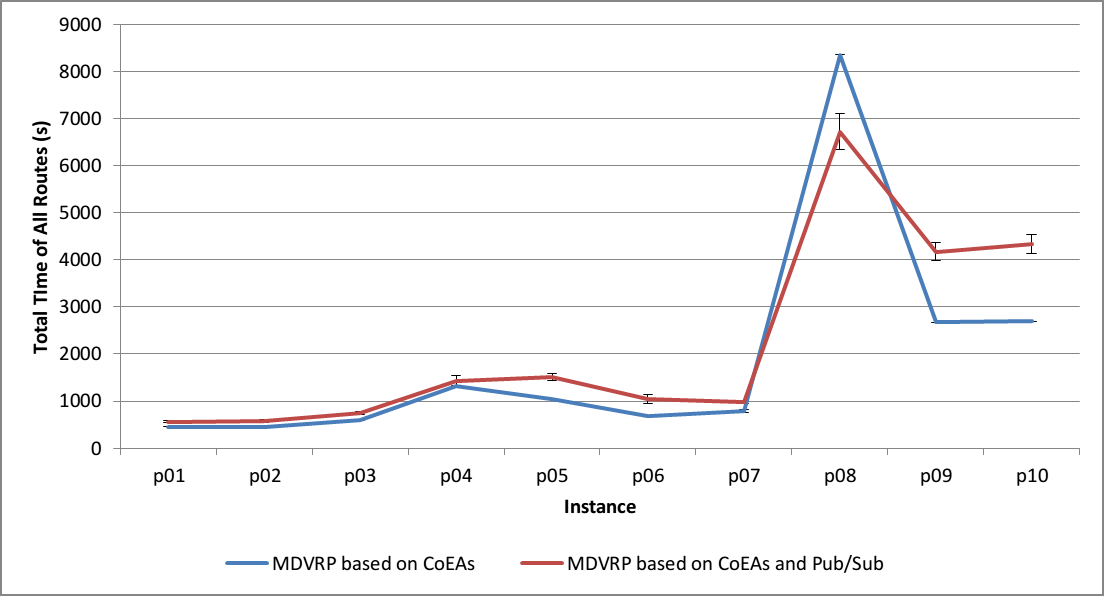
\includegraphics[width=\textwidth]{Resources/Images/test_result_10_cordeau_total_time}
	\caption{Rata-rata total waktu seluruh rute dari 5 kali pengujian tanpa \textit{service time} pada data Cordeau}
	\label{fig:test_result_10_cordeau_total_time}
\end{figure}


\begin{longtable}[!]{c|rrrr}
	\caption{Perbandingan standar deviasi total waktu setiap rute dari pengujian tanpa \textit{service time} pada data cordeau P01 (detik)}
	\label{tbl:test_result_p01_notw_standard_deviation_of_total_time}\\
	\toprule
	\textit{Pengujian ke} & \MyHead{4cm}{MDVRP berbasis CoEAs} & \MyHead{4cm}{MDVRP berbasis CoEAs dan Pub/Sub} \\ 
	\midrule
	\endfirsthead
	\toprule
	\textit{Pengujian ke} & \MyHead{4cm}{MDVRP berbasis CoEAs} & \MyHead{4cm}{MDVRP berbasis CoEAs dan Pub/Sub} \\ 
	\midrule
	\endhead
	\bottomrule
	\endfoot
	1 & 27.24 & 20.84 \\
	2 & 27.24 & 6.64  \\
	3 & 27.24 & 12.67 \\
	4 & 26.45 & 19.45 \\
	5 & 27.06 & 15.2 \\
\end{longtable}


\begin{longtable}[!]{c|rrrr}
	\caption{Perbandingan standar deviasi total waktu setiap rute dari pengujian tanpa \textit{service time} pada data cordeau P02 (detik)}
	\label{tbl:test_result_p02_notw_standard_deviation_of_total_time}\\
	\toprule
	\textit{Pengujian ke} & \MyHead{4cm}{MDVRP berbasis CoEAs} & \MyHead{4cm}{MDVRP berbasis CoEAs dan Pub/Sub} \\ 
	\midrule
	\endfirsthead
	\toprule
	\textit{Pengujian ke} & \MyHead{4cm}{MDVRP berbasis CoEAs} & \MyHead{4cm}{MDVRP berbasis CoEAs dan Pub/Sub} \\ 
	\midrule
	\endhead
	\bottomrule
	\endfoot
	1 & 25.9  & 13.32 \\
	2 & 27.24 & 18.2  \\
	3 & 27.93 & 12.89 \\
	4 & 27.24 & 35.56 \\
	5 & 27.24 & 37.51 \\
\end{longtable}


\begin{longtable}[!]{c|rrrr}
	\caption{Perbandingan standar deviasi total waktu setiap rute dari pengujian tanpa \textit{service time} pada data cordeau P03 (detik)}
	\label{tbl:test_result_p03_notw_standard_deviation_of_total_time}\\
	\toprule
	\textit{Pengujian ke} & \MyHead{4cm}{MDVRP berbasis CoEAs} & \MyHead{4cm}{MDVRP berbasis CoEAs dan Pub/Sub} \\ 
	\midrule
	\endfirsthead
	\toprule
	\textit{Pengujian ke} & \MyHead{4cm}{MDVRP berbasis CoEAs} & \MyHead{4cm}{MDVRP berbasis CoEAs dan Pub/Sub} \\ 
	\midrule
	\endhead
	\bottomrule
	\endfoot
	1 & 32.47 & 20.09 \\
	2 & 32.47 & 27.46 \\
	3 & 37.66 & 34.13 \\
	4 & 32.47 & 31.17 \\
	5 & 38.68 & 36.88 \\
\end{longtable}


\begin{longtable}[!]{c|rrrr}
	\caption{Perbandingan standar deviasi total waktu setiap rute dari pengujian tanpa \textit{service time} pada data cordeau P04 (detik)}
	\label{tbl:test_result_p04_notw_standard_deviation_of_total_time}\\
	\toprule
	\textit{Pengujian ke} & \MyHead{4cm}{MDVRP berbasis CoEAs} & \MyHead{4cm}{MDVRP berbasis CoEAs dan Pub/Sub} \\ 
	\midrule
	\endfirsthead
	\toprule
	\textit{Pengujian ke} & \MyHead{4cm}{MDVRP berbasis CoEAs} & \MyHead{4cm}{MDVRP berbasis CoEAs dan Pub/Sub} \\ 
	\midrule
	\endhead
	\bottomrule
	\endfoot
	1 & 199.16 & 16.1   \\
	2 & 199.16 & 64.51  \\
	3 & 199.16 & 25.62  \\
	4 & 199.16 & 25.12  \\
	5 & 199.16 & 183.82 \\
\end{longtable}


\begin{longtable}[!]{c|rrrr}
	\caption{Perbandingan standar deviasi total waktu setiap rute dari pengujian tanpa \textit{service time} pada data cordeau P05 (detik)}
	\label{tbl:test_result_p05_notw_standard_deviation_of_total_time}\\
	\toprule
	\textit{Pengujian ke} & \MyHead{4cm}{MDVRP berbasis CoEAs} & \MyHead{4cm}{MDVRP berbasis CoEAs dan Pub/Sub} \\ 
	\midrule
	\endfirsthead
	\toprule
	\textit{Pengujian ke} & \MyHead{4cm}{MDVRP berbasis CoEAs} & \MyHead{4cm}{MDVRP berbasis CoEAs dan Pub/Sub} \\ 
	\midrule
	\endhead
	\bottomrule
	\endfoot
	1 & 76.61 & 1.09   \\
	2 & 76.61 & 11.62  \\
	3 & 76.61 & 91.1   \\
	4 & 76.61 & 149.23 \\
	5 & 76.61 & 149.23 \\
\end{longtable}


\begin{longtable}[!]{c|rrrr}
	\caption{Perbandingan standar deviasi total waktu setiap rute dari pengujian tanpa \textit{service time} pada data cordeau P06 (detik)}
	\label{tbl:test_result_p06_notw_standard_deviation_of_total_time}\\
	\toprule
	\textit{Pengujian ke} & \MyHead{4cm}{MDVRP berbasis CoEAs} & \MyHead{4cm}{MDVRP berbasis CoEAs dan Pub/Sub} \\ 
	\midrule
	\endfirsthead
	\toprule
	\textit{Pengujian ke} & \MyHead{4cm}{MDVRP berbasis CoEAs} & \MyHead{4cm}{MDVRP berbasis CoEAs dan Pub/Sub} \\ 
	\midrule
	\endhead
	\bottomrule
	\endfoot
	1 & 57.15 & 48.82 \\
	2 & 57.15 & 17.55 \\
	3 & 57.15 & 46.44 \\
	4 & 57.15 & 39.64 \\
	5 & 57.15 & 35.93 \\
\end{longtable}


\begin{longtable}[!]{c|rrrr}
	\caption{Perbandingan standar deviasi total waktu setiap rute dari pengujian tanpa \textit{service time} pada data cordeau P07 (detik)}
	\label{tbl:test_result_p07_notw_standard_deviation_of_total_time}\\
	\toprule
	\textit{Pengujian ke} & \MyHead{4cm}{MDVRP berbasis CoEAs} & \MyHead{4cm}{MDVRP berbasis CoEAs dan Pub/Sub} \\ 
	\midrule
	\endfirsthead
	\toprule
	\textit{Pengujian ke} & \MyHead{4cm}{MDVRP berbasis CoEAs} & \MyHead{4cm}{MDVRP berbasis CoEAs dan Pub/Sub} \\ 
	\midrule
	\endhead
	\bottomrule
	\endfoot
	1 & 29.08 & 67.27 \\
	2 & 42.64 & 49.93 \\
	3 & 42.64 & 27.02 \\
	4 & 42.64 & 24.19 \\
	5 & 45.48 & 32.57 \\
\end{longtable}


\begin{longtable}[!]{c|rrrr}
	\caption{Perbandingan standar deviasi total waktu setiap rute dari pengujian tanpa \textit{service time} pada data cordeau P08 (detik)}
	\label{tbl:test_result_p08_notw_standard_deviation_of_total_time}\\
	\toprule
	\textit{Pengujian ke} & \MyHead{4cm}{MDVRP berbasis CoEAs} & \MyHead{4cm}{MDVRP berbasis CoEAs dan Pub/Sub} \\ 
	\midrule
	\endfirsthead
	\toprule
	\textit{Pengujian ke} & \MyHead{4cm}{MDVRP berbasis CoEAs} & \MyHead{4cm}{MDVRP berbasis CoEAs dan Pub/Sub} \\ 
	\midrule
	\endhead
	\bottomrule
	\endfoot
	1 & 1962.81 & 228.95 \\
	2 & 1962.81 & 208.59 \\
	3 & 1962.81 & 296.74 \\
	4 & 1962.81 & 48.84  \\
	5 & 1962.81 & 126.74 \\
\end{longtable}


\begin{longtable}[!]{c|rrrr}
	\caption{Perbandingan standar deviasi total waktu setiap rute dari pengujian tanpa \textit{service time} pada data cordeau P09 (detik)}
	\label{tbl:test_result_p09_notw_standard_deviation_of_total_time}\\
	\toprule
	\textit{Pengujian ke} & \MyHead{4cm}{MDVRP berbasis CoEAs} & \MyHead{4cm}{MDVRP berbasis CoEAs dan Pub/Sub} \\ 
	\midrule
	\endfirsthead
	\toprule
	\textit{Pengujian ke} & \MyHead{4cm}{MDVRP berbasis CoEAs} & \MyHead{4cm}{MDVRP berbasis CoEAs dan Pub/Sub} \\ 
	\midrule
	\endhead
	\bottomrule
	\endfoot
	1 & 208.99 & 117.76 \\
	2 & 208.99 & 164.76 \\
	3 & 208.99 & 78.29  \\
	4 & 208.99 & 68.88  \\
	5 & 208.99 & 18.57 \\
\end{longtable}


\begin{longtable}[!]{c|rrrr}
	\caption{Perbandingan standar deviasi total waktu setiap rute dari pengujian tanpa \textit{service time} pada data cordeau P10 (detik)}
	\label{tbl:test_result_p10_notw_standard_deviation_of_total_time}\\
	\toprule
	\textit{Pengujian ke} & \MyHead{4cm}{MDVRP berbasis CoEAs} & \MyHead{4cm}{MDVRP berbasis CoEAs dan Pub/Sub} \\ 
	\midrule
	\endfirsthead
	\toprule
	\textit{Pengujian ke} & \MyHead{4cm}{MDVRP berbasis CoEAs} & \MyHead{4cm}{MDVRP berbasis CoEAs dan Pub/Sub} \\ 
	\midrule
	\endhead
	\bottomrule
	\endfoot
	1 & 130.08 & 200.31 \\
	2 & 130.08 & 237.45 \\
	3 & 130.08 & 106.7  \\
	4 & 130.08 & 219.08 \\
	5 & 130.08 & 94.16 \\
\end{longtable}


\begin{longtable}[!]{c|rrrr}
	\caption{Rata-rata standar deviasi total waktu setiap rute dari 5 kali pengujian tanpa \textit{service time} pada data cordeau (detik)}
	\label{tbl:test_result_cordeau_notw_standard_deviation_of_total_time}\\
	\toprule
	\textit{\textit{Instance}} & \MyHead{4cm}{MDVRP berbasis CoEAs} & \MyHead{4cm}{MDVRP berbasis CoEAs dan Pub/Sub} \\ 
	\midrule
	\endfirsthead
	\toprule
	\textit{\textit{Instance}} & \MyHead{4cm}{MDVRP berbasis CoEAs} & \MyHead{4cm}{MDVRP berbasis CoEAs dan Pub/Sub} \\ 
	\midrule
	\endhead
	\bottomrule
	\endfoot
	p01 & 27.05    & \textbf{14.96}  \\
	p02 & 27.11    & \textbf{23.50}  \\
	p03 & 34.75    & \textbf{29.95}  \\
	p04 & 199.16   & \textbf{63.03}  \\
	p05 & \textbf{76.61}    & 80.45  \\
	p06 & 57.15    & \textbf{37.68}  \\
	p07 & 40.50    & \textbf{40.20}  \\
	p08 & 1,962.81 & \textbf{181.97} \\
	p09 & 208.99   & \textbf{89.65}  \\
	p10 & \textbf{130.08}   & 171.54 \\
\end{longtable}


\begin{figure}[!]
	\centering
	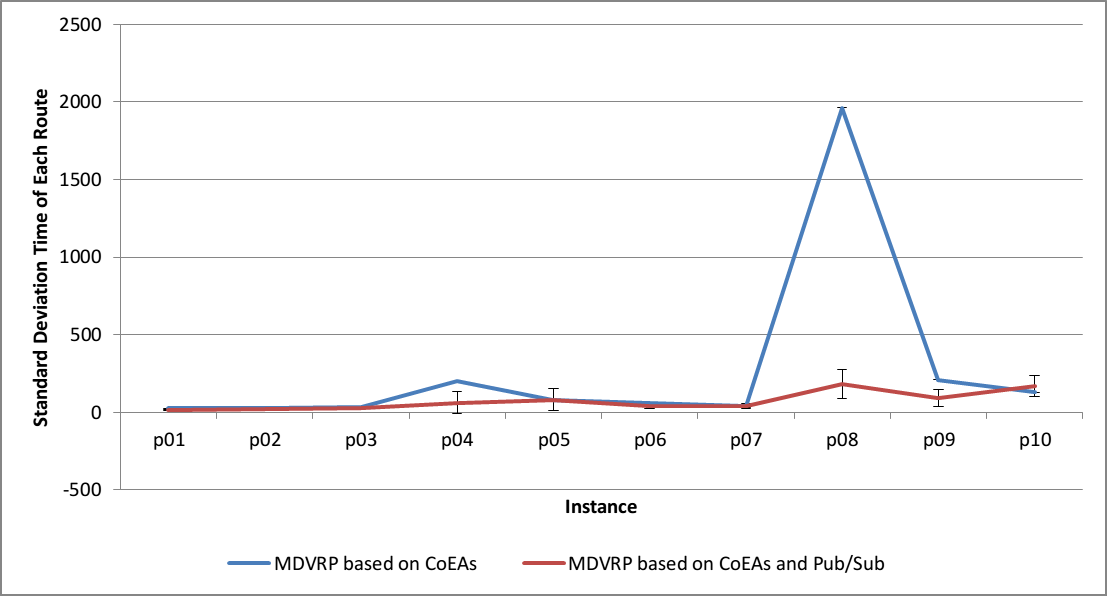
\includegraphics[width=\textwidth]{Resources/Images/test_result_10_cordeau_standard_deviation}
	\caption{Rata-rata standar deviasi total waktu waktu setiap rute dari 5 kali pengujian tanpa \textit{service time} pada data Cordeau}
	\label{fig:test_result_10_cordeau_standard_deviation}
\end{figure}


%-----------------------------------------------------------------------------%
\subsubsection{Pengujian Kondisi Normal dengan \textit{Service Time}}
\label{ssec:test-normal-service-time}
%-----------------------------------------------------------------------------%
Skenario pengujian kondisi normal dimaksudkan untuk membandingkan sistem yang dijalankan pada kondisi normal, dimana tidak ada sesuatupun yang menyebabkan penundaaan. Pengujian kondisi ini dilakukan untuk tiap-tiap data Cordeau (P01 sampai P10) dan data lapangan. 


Data \textit{service time} digenerate secara random dengan mengikuti komposisi dari \citep{sudman_time_1965}, yaitu:
\begin{enumerate}
	\item 21 persen dari total waktu digunakan untuk perpindahan antar segmen, 
	\item 15 persen dari total waktu digunakan untuk perpindahan antar rumah tangga dalam segmen, 
	\item 37 persen dari total waktu digunakan untuk wawancara seluruh responden, dan 
	\item 27 persen untuk hal-hal yang lain, seperti pengenalan wilayah dan perbaikan data.
\end{enumerate}
\textit{Service time} merupakan gabungan dari waktu perpindahan antar rumah tangga dan waktu wawancara. Meskipun komposisi waktu \citep{sudman_time_1965} dinilai kurang relevan, akan tetapi masih dapat digunakan sebagai dasar untuk men-\textit{generate} \textit{service time}. Adapun penggunaan komposisi waktu yang lebih relevan terdapat pada \autoref{sssec:test-delay-service-time}.


Berikut adalah komposisi dari tiap-tiap \textit{instance} yang diujicobakan:
\begin{enumerate}
	\item Instance P01 terdiri dari 50 \textit{customer} dan 5 \textit{vehicle}, lama wawancara 27.58 menit dengan standar deviasi 12.13 menit.
	\item Instance P02 terdiri dari 50 \textit{customer} dan 4 \textit{vehicle}, lama wawancara 27.58 menit dengan standar deviasi 12.13 menit.
	\item Instance P03 terdiri dari 75 \textit{customer} dan 5 \textit{vehicle}, lama wawancara 27.58 menit dengan standar deviasi 12.13 menit.
	\item Instance P04 terdiri dari 100 \textit{customer} dan 2 \textit{vehicle}, lama wawancara 27.58 menit dengan standar deviasi 12.13 menit.
	\item Instance P05 terdiri dari 100 \textit{customer} dan 2 \textit{vehicle}, lama wawancara 27.58 menit dengan standar deviasi 12.13 menit.
	\item Instance P06 terdiri dari 100 \textit{customer} dan 3 \textit{vehicle}, lama wawancara 27.58 menit dengan standar deviasi 12.13 menit.
	\item Instance P07 terdiri dari 100 \textit{customer} dan 4 \textit{vehicle}, lama wawancara 27.58 menit dengan standar deviasi 12.13 menit.
	\item Instance P08 terdiri dari 249 \textit{customer} dan 2 \textit{vehicle}, lama wawancara 27.58 menit dengan standar deviasi 12.13 menit.
	\item Instance P09 terdiri dari 249 \textit{customer} dan 3 \textit{vehicle}, lama wawancara 27.58 menit dengan standar deviasi 12.13 menit.
	\item Instance P10 terdiri dari 249 \textit{customer} dan 4 \textit{vehicle}, lama wawancara 27.58 menit dengan standar deviasi 12.13 menit.
\end{enumerate}
Adapun data lapangan memiliki komposisi sebagai berikut:
\begin{enumerate}
	\item Instance TW1 terdiri dari 182 \textit{customer} dan 15 \textit{vehicle}, lama wawancara 27.58 menit dengan standar deviasi 4,13 menit.
	\item Instance TW2 terdiri dari 182 \textit{customer} dan 15 \textit{vehicle}, lama wawancara 71.58 menit dengan standar deviasi 12.16 menit.
	\item Instance TW3 terdiri dari 182 \textit{customer} dan 15 \textit{vehicle}, lama wawancara 27.35 menit dengan standar deviasi 25.34 menit.
	\item Instance TW4 terdiri dari 182 \textit{customer} dan 15 \textit{vehicle}, lama wawancara 71.58 menit dengan standar deviasi 56.87 menit.
\end{enumerate}


Setiap \textit{instance} data diuji sebanyak 5 (lima) kali untuk membuktikan bahwa hasil yang diperoleh konsisten. Dari hasil simulasi, diperoleh rute untuk tiap-tiap \textit{instance} Cordeau sebagaimana digambarkan pada \hyperref[ch:test_result_cordeau_tw]{Lampiran 2}. Kemudian dari seluruh rute yang diperoleh, dikalkulasi waktu total untuk tiap-tiap rute, waktu total dari seluruh rute pada sebuah \textit{instance}, dan standar deviasi total waktu dari seluruh rute untuk setiap \textit{instance}, sebagaimana cara yang dijelaskan pada \autoref{sssec:metric}. 


Berdasarkan \autoref{fig:test_result_10_cordeau_tw_total_time}, diperoleh hasil bahwa dengan menggunakan sistem usulan, 9 dari 10 \textit{instance} menghasilkan \textbf{total waktu} yang lebih kecil, meskipun selisihnya sangat kecil, seperti dirincikan pada \autoref{tbl:test_result_cordeau_tw_total_time}. Sementara dari sisi \textbf{standar deviasi total waktu dari seluruh rute}, (\autoref{fig:test_result_10_cordeau_tw_standard_deviation}), diperoleh hasil bahwa setiap \textit{instance} yang dijalankan pada sistem usulan menghasilkan standar deviasi yang lebih kecil dibandingkan \textit{instance} yang sama dengan sistem pembanding (\autoref{tbl:test_result_cordeau_tw_standard_deviation_of_total_time}). Hal ini semakin mempertegas kesimpulan dari pengujian sebelumnya yang menyatakan bahwa program usulan berupa MDVRP berbasis CoEAs dan mekansime \textit{publish/subscribe} lebih efisien dan menghasilkan rute dengan beban tugas yang lebih merata antar petugas. Hal ini berdampak positif kepada total waktu seluruh kegiatan dengan sistem usulan menjadi lebih pendek dibandingkan sistem pembanding.


\begin{longtable}[!]{c|rrrr}
	\caption{Perbandingan total waktu seluruh rute dari pengujian dengan \textit{service time} pada data cordeau P01 (detik)}
	\label{tbl:test_result_p01_tw_total_time}\\
	\toprule
	\textit{Pengujian ke} & \MyHead{4cm}{MDVRP berbasis CoEAs} & \MyHead{4cm}{MDVRP berbasis CoEAs dan Pub/Sub} \\ 
	\midrule
	\endfirsthead
	\toprule
	\textit{Pengujian ke} & \MyHead{4cm}{MDVRP berbasis CoEAs} & \MyHead{4cm}{MDVRP berbasis CoEAs dan Pub/Sub} \\ 
	\midrule
	\endhead
	\bottomrule
	\endfoot
	1 & 824.513,17 & 824.649,98 \\
	2  & 824.513,17 & 824.665,06 \\
	3  & 824.513,17 & 824.642,97 \\
	4  & 824.513,17 & 824.610,03 \\
	5  & 824.514,07 & 824.636,45 \\
\end{longtable}


\begin{longtable}[!]{c|rrrr}
	\caption{Perbandingan total waktu seluruh rute dari pengujian dengan \textit{service time} pada data cordeau P02 (detik)}
	\label{tbl:test_result_p02_tw_total_time}\\
	\toprule
	\textit{Pengujian ke} & \MyHead{4cm}{MDVRP berbasis CoEAs} & \MyHead{4cm}{MDVRP berbasis CoEAs dan Pub/Sub} \\ 
	\midrule
	\endfirsthead
	\toprule
	\textit{Pengujian ke} & \MyHead{4cm}{MDVRP berbasis CoEAs} & \MyHead{4cm}{MDVRP berbasis CoEAs dan Pub/Sub} \\ 
	\midrule
	\endhead
	\bottomrule
	\endfoot
	1 & 805.990,03 & 806.090,97 \\
	2  & 805.995,51 & 806.149,31 \\
	3  & 805.994,30 & 806.139,29 \\
	4  & 805.990,03 & 806.096,73 \\
	5  & 805.990,03 & 806.149,57 \\
\end{longtable}


\begin{longtable}[!]{c|rrrr}
	\caption{Perbandingan total waktu seluruh rute dari pengujian dengan \textit{service time} pada data cordeau P03 (detik)}
	\label{tbl:test_result_p03_tw_total_time}\\
	\toprule
	\textit{Pengujian ke} & \MyHead{4cm}{MDVRP berbasis CoEAs} & \MyHead{4cm}{MDVRP berbasis CoEAs dan Pub/Sub} \\ 
	\midrule
	\endfirsthead
	\toprule
	\textit{Pengujian ke} & \MyHead{4cm}{MDVRP berbasis CoEAs} & \MyHead{4cm}{MDVRP berbasis CoEAs dan Pub/Sub} \\ 
	\midrule
	\endhead
	\bottomrule
	\endfoot
	1 & 1.256.883,28 & 1.257.044,56 \\
	2  & 1.256.878,59 & 1.257.003,13 \\
	3  & 1.256.880,05 & 1.257.052,22 \\
	4  & 1.256.883,28 & 1.257.165,57 \\
	5  & 1.256.883,28 & 1.257.075,47 \\
\end{longtable}


\begin{longtable}[!]{c|rrrr}
	\caption{Perbandingan total waktu seluruh rute dari pengujian dengan \textit{service time} pada data cordeau P04 (detik)}
	\label{tbl:test_result_p04_tw_total_time}\\
	\toprule
	\textit{Pengujian ke} & \MyHead{4cm}{MDVRP berbasis CoEAs} & \MyHead{4cm}{MDVRP berbasis CoEAs dan Pub/Sub} \\ 
	\midrule
	\endfirsthead
	\toprule
	\textit{Pengujian ke} & \MyHead{4cm}{MDVRP berbasis CoEAs} & \MyHead{4cm}{MDVRP berbasis CoEAs dan Pub/Sub} \\ 
	\midrule
	\endhead
	\bottomrule
	\endfoot
	1 & 1.642.834,05 & 1.643.051,50 \\
	2  & 1.642.834,05 & 1.642.910,58 \\
	3  & 1.642.834,05 & 1.642.978,41 \\
	4  & 1.642.834,05 & 1.642.960,50 \\
	5  & 1.642.834,05 & 1.642.920,79 \\
\end{longtable}


\begin{longtable}[!]{c|rrrr}
	\caption{Perbandingan total waktu seluruh rute dari pengujian dengan \textit{service time} pada data cordeau P05 (detik)}
	\label{tbl:test_result_p05_tw_total_time}\\
	\toprule
	\textit{Pengujian ke} & \MyHead{4cm}{MDVRP berbasis CoEAs} & \MyHead{4cm}{MDVRP berbasis CoEAs dan Pub/Sub} \\ 
	\midrule
	\endfirsthead
	\toprule
	\textit{Pengujian ke} & \MyHead{4cm}{MDVRP berbasis CoEAs} & \MyHead{4cm}{MDVRP berbasis CoEAs dan Pub/Sub} \\ 
	\midrule
	\endhead
	\bottomrule
	\endfoot
	1 & 1.654.118,92 & 1.654.511,94 \\
	2  & 1.654.118,92 & 1.654.689,45 \\
	3  & 1.654.118,92 & 1.654.583,63 \\
	4  & 1.654.118,92 & 1.654.408,94 \\
	5  & 1.654.118,92 & 1.654.744,01 \\
\end{longtable}


\begin{longtable}[!]{c|rrrr}
	\caption{Perbandingan total waktu seluruh rute dari pengujian dengan \textit{service time} pada data cordeau P06 (detik)}
	\label{tbl:test_result_p06_tw_total_time}\\
	\toprule
	\textit{Pengujian ke} & \MyHead{4cm}{MDVRP berbasis CoEAs} & \MyHead{4cm}{MDVRP berbasis CoEAs dan Pub/Sub} \\ 
	\midrule
	\endfirsthead
	\toprule
	\textit{Pengujian ke} & \MyHead{4cm}{MDVRP berbasis CoEAs} & \MyHead{4cm}{MDVRP berbasis CoEAs dan Pub/Sub} \\ 
	\midrule
	\endhead
	\bottomrule
	\endfoot
	1 & 1.634.803,49 & 1.635.193,62 \\
	2  & 1.634.803,49 & 1.635.190,04 \\
	3  & 1.634.803,49 & 1.635.177,49 \\
	4  & 1.634.803,49 & 1.635.165,26 \\
	5  & 1.634.803,49 & 1.635.057,02 \\
\end{longtable}


\begin{longtable}[!]{c|rrrr}
	\caption{Perbandingan total waktu seluruh rute dari pengujian dengan \textit{service time} pada data cordeau P07 (detik)}
	\label{tbl:test_result_p07_tw_total_time}\\
	\toprule
	\textit{Pengujian ke} & \MyHead{4cm}{MDVRP berbasis CoEAs} & \MyHead{4cm}{MDVRP berbasis CoEAs dan Pub/Sub} \\ 
	\midrule
	\endfirsthead
	\toprule
	\textit{Pengujian ke} & \MyHead{4cm}{MDVRP berbasis CoEAs} & \MyHead{4cm}{MDVRP berbasis CoEAs dan Pub/Sub} \\ 
	\midrule
	\endhead
	\bottomrule
	\endfoot
	1 & 1.639.779,18 & 1.639.996,92 \\
	2  & 1.639.759,38 & 1.639.875,94 \\
	3  & 1.639.759,38 & 1.639.951,64 \\
	4  & 1.639.759,38 & 1.639.955,73 \\
	5  & 1.639.771,58 & 1.639.964,31 \\
\end{longtable}


\begin{longtable}[!]{c|rrrr}
	\caption{Perbandingan total waktu seluruh rute dari pengujian dengan \textit{service time} pada data cordeau P08 (detik)}
	\label{tbl:test_result_p08_tw_total_time}\\
	\toprule
	\textit{Pengujian ke} & \MyHead{4cm}{MDVRP berbasis CoEAs} & \MyHead{4cm}{MDVRP berbasis CoEAs dan Pub/Sub} \\ 
	\midrule
	\endfirsthead
	\toprule
	\textit{Pengujian ke} & \MyHead{4cm}{MDVRP berbasis CoEAs} & \MyHead{4cm}{MDVRP berbasis CoEAs dan Pub/Sub} \\ 
	\midrule
	\endhead
	\bottomrule
	\endfoot
	1 & 4.133.012,69 & 4.131.449,89 \\
	2  & 4.133.012,69 & 4.130.779,21 \\
	3  & 4.133.012,69 & 4.131.259,75 \\
	4  & 4.133.012,69 & 4.130.968,21 \\
	5  & 4.133.012,69 & 4.131.105,47 \\
\end{longtable}


\begin{longtable}[!]{c|rrrr}
	\caption{Perbandingan total waktu seluruh rute dari pengujian dengan \textit{service time} pada data cordeau P09 (detik)}
	\label{tbl:test_result_p09_tw_total_time}\\
	\toprule
	\textit{Pengujian ke} & \MyHead{4cm}{MDVRP berbasis CoEAs} & \MyHead{4cm}{MDVRP berbasis CoEAs dan Pub/Sub} \\ 
	\midrule
	\endfirsthead
	\toprule
	\textit{Pengujian ke} & \MyHead{4cm}{MDVRP berbasis CoEAs} & \MyHead{4cm}{MDVRP berbasis CoEAs dan Pub/Sub} \\ 
	\midrule
	\endhead
	\bottomrule
	\endfoot
	1 & 4.132.046,12 & 4.133.516,34 \\
	2  & 4.132.046,12 & 4.133.430,95 \\
	3  & 4.132.046,12 & 4.133.790,81 \\
	4  & 4.132.046,12 & 4.133.604,83 \\
	5  & 4.132.046,12 & 4.133.541,31 \\
\end{longtable}


\begin{longtable}[!]{c|rrrr}
	\caption{Perbandingan total waktu seluruh rute dari pengujian dengan \textit{service time} pada data cordeau P10 (detik)}
	\label{tbl:test_result_p10_tw_total_time}\\
	\toprule
	\textit{Pengujian ke} & \MyHead{4cm}{MDVRP berbasis CoEAs} & \MyHead{4cm}{MDVRP berbasis CoEAs dan Pub/Sub} \\ 
	\midrule
	\endfirsthead
	\toprule
	\textit{Pengujian ke} & \MyHead{4cm}{MDVRP berbasis CoEAs} & \MyHead{4cm}{MDVRP berbasis CoEAs dan Pub/Sub} \\ 
	\midrule
	\endhead
	\bottomrule
	\endfoot
	1 & 4.115.466,02 & 4.117.128,75 \\
	2  & 4.115.466,02 & 4.117.017,19 \\
	3  & 4.115.466,02 & 4.117.045,17 \\
	4  & 4.115.466,02 & 4.117.007,61 \\
	5  & 4.115.466,02 & 4.117.283,84 \\
\end{longtable}


\begin{longtable}[!]{c|rrrr}
	\caption{Rata-rata total waktu seluruh rute dari 5 kali pengujian dengan \textit{service time} pada data cordeau (detik)}
	\label{tbl:test_result_cordeau_tw_total_time}\\
	\toprule
	\textit{\textit{Instance}} & \MyHead{4cm}{MDVRP berbasis CoEAs} & \MyHead{4cm}{MDVRP berbasis CoEAs dan Pub/Sub} \\ 
	\midrule
	\endfirsthead
	\toprule
	\textit{\textit{Instance}} & \MyHead{4cm}{MDVRP berbasis CoEAs} & \MyHead{4cm}{MDVRP berbasis CoEAs dan Pub/Sub} \\ 
	\midrule
	\endhead
	\bottomrule
	\endfoot
	p01 & \textbf{824.513,35}   & 824.640,90   \\
	p02  & \textbf{805.991,98}   & 806.125,17   \\
	p03  & \textbf{1.256.881,70} & 1.257.068,19 \\
	p04  & \textbf{1.642.834,05} & 1.642.964,36 \\
	p05  & \textbf{1.654.118,92} & 1.654.587,59 \\
	p06  & \textbf{1.634.803,49} & 1.635.156,69 \\
	p07  & \textbf{1.639.765,78} & 1.639.948,91 \\
	p08  & 4.133.012,69 & \textbf{4.131.112,51} \\
	p09  & \textbf{4.132.046,12} & 4.133.576,85 \\
	p10  & \textbf{4.115.466,02} & 4.117.096,51 \\
\end{longtable}


\begin{figure}[!]
	\centering
	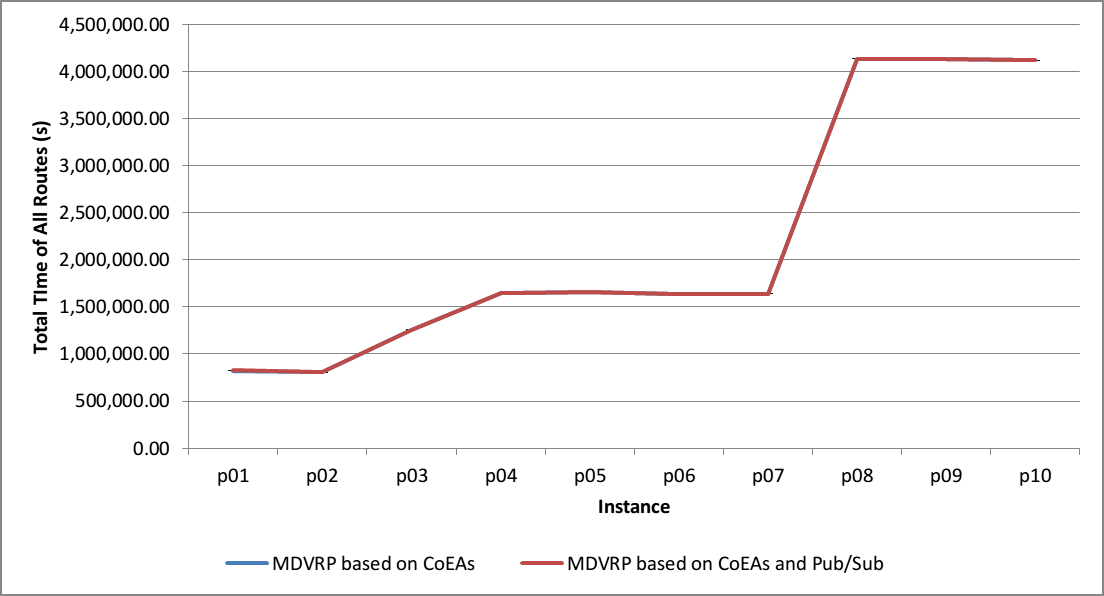
\includegraphics[width=\textwidth]{Resources/Images/test_result_10_cordeau_tw_total_time}
	\caption{Rata-rata total waktu seluruh rute dari 5 kali pengujian dengan \textit{service time} pada data Cordeau}
	\label{fig:test_result_10_cordeau_tw_total_time}
\end{figure}


\begin{longtable}[!]{c|rrrr}
	\caption{Perbandingan standar deviasi total waktu setiap rute dari pengujian dengan \textit{service time} pada data cordeau P01 (detik)}
	\label{tbl:test_result_p01_tw_standard_deviation_of_total_time}\\
	\toprule
	\textit{Pengujian ke} & \MyHead{4cm}{MDVRP berbasis CoEAs} & \MyHead{4cm}{MDVRP berbasis CoEAs dan Pub/Sub} \\ 
	\midrule
	\endfirsthead
	\toprule
	\textit{Pengujian ke} & \MyHead{4cm}{MDVRP berbasis CoEAs} & \MyHead{4cm}{MDVRP berbasis CoEAs dan Pub/Sub} \\ 
	\midrule
	\endhead
	\bottomrule
	\endfoot
	1 & 44.165,10 & 12.539,43 \\
	2  & 44.165,10 & 6.692,99  \\
	3  & 44.165,10 & 4.852,02  \\
	4  & 44.165,10 & 8.990,18  \\
	5  & 44.165,01 & 14.344,51 \\
\end{longtable}


\begin{longtable}[!]{c|rrrr}
	\caption{Perbandingan standar deviasi total waktu setiap rute dari pengujian dengan \textit{service time} pada data cordeau P02 (detik)}
	\label{tbl:test_result_p02_tw_standard_deviation_of_total_time}\\
	\toprule
	\textit{Pengujian ke} & \MyHead{4cm}{MDVRP berbasis CoEAs} & \MyHead{4cm}{MDVRP berbasis CoEAs dan Pub/Sub} \\ 
	\midrule
	\endfirsthead
	\toprule
	\textit{Pengujian ke} & \MyHead{4cm}{MDVRP berbasis CoEAs} & \MyHead{4cm}{MDVRP berbasis CoEAs dan Pub/Sub} \\ 
	\midrule
	\endhead
	\bottomrule
	\endfoot
	1 & 37.666,96 & 12.322,08 \\
	2  & 37.666,70 & 7.639,29  \\
	3  & 37.666,76 & 11.327,81 \\
	4  & 37.666,96 & 12.838,96 \\
	5  & 37.666,96 & 15.875,32 \\
\end{longtable}


\begin{longtable}[!]{c|rrrr}
	\caption{Perbandingan standar deviasi total waktu setiap rute dari pengujian dengan \textit{service time} pada data cordeau P03 (detik)}
	\label{tbl:test_result_p03_tw_standard_deviation_of_total_time}\\
	\toprule
	\textit{Pengujian ke} & \MyHead{4cm}{MDVRP berbasis CoEAs} & \MyHead{4cm}{MDVRP berbasis CoEAs dan Pub/Sub} \\ 
	\midrule
	\endfirsthead
	\toprule
	\textit{Pengujian ke} & \MyHead{4cm}{MDVRP berbasis CoEAs} & \MyHead{4cm}{MDVRP berbasis CoEAs dan Pub/Sub} \\ 
	\midrule
	\endhead
	\bottomrule
	\endfoot
	1 & 57.486,44 & 13.271,86 \\
	2  & 65.668,31 & 17.904,54 \\
	3  & 65.667,82 & 11.745,67 \\
	4  & 57.486,44 & 8.612,42  \\
	5  & 57.486,44 & 19.039,83 \\
\end{longtable}


\begin{longtable}[!]{c|rrrr}
	\caption{Perbandingan standar deviasi total waktu setiap rute dari pengujian dengan \textit{service time} pada data cordeau P04 (detik)}
	\label{tbl:test_result_p04_tw_standard_deviation_of_total_time}\\
	\toprule
	\textit{Pengujian ke} & \MyHead{4cm}{MDVRP berbasis CoEAs} & \MyHead{4cm}{MDVRP berbasis CoEAs dan Pub/Sub} \\ 
	\midrule
	\endfirsthead
	\toprule
	\textit{Pengujian ke} & \MyHead{4cm}{MDVRP berbasis CoEAs} & \MyHead{4cm}{MDVRP berbasis CoEAs dan Pub/Sub} \\ 
	\midrule
	\endhead
	\bottomrule
	\endfoot
	1 & 148.762,94 & 4.719,26  \\
	2  & 148.762,94 & 7.750,10  \\
	3  & 148.762,94 & 2.543,91  \\
	4  & 148.762,94 & 19.527,95 \\
	5  & 148.762,94 & 9.056,45  \\
\end{longtable}


\begin{longtable}[!]{c|rrrr}
	\caption{Perbandingan standar deviasi total waktu setiap rute dari pengujian dengan \textit{service time} pada data cordeau P05 (detik)}
	\label{tbl:test_result_p05_tw_standard_deviation_of_total_time}\\
	\toprule
	\textit{Pengujian ke} & \MyHead{4cm}{MDVRP berbasis CoEAs} & \MyHead{4cm}{MDVRP berbasis CoEAs dan Pub/Sub} \\ 
	\midrule
	\endfirsthead
	\toprule
	\textit{Pengujian ke} & \MyHead{4cm}{MDVRP berbasis CoEAs} & \MyHead{4cm}{MDVRP berbasis CoEAs dan Pub/Sub} \\ 
	\midrule
	\endhead
	\bottomrule
	\endfoot
	1 & 154.028,63 & 22.469,85 \\
	2  & 154.028,63 & 5.169,54  \\
	3  & 154.028,63 & 5.868,09  \\
	4  & 154.028,63 & 12.326,93 \\
	5  & 154.028,63 & 24.263,43 \\
\end{longtable}


\begin{longtable}[!]{c|rrrr}
	\caption{Perbandingan standar deviasi total waktu setiap rute dari pengujian dengan \textit{service time} pada data cordeau P06 (detik)}
	\label{tbl:test_result_p06_tw_standard_deviation_of_total_time}\\
	\toprule
	\textit{Pengujian ke} & \MyHead{4cm}{MDVRP berbasis CoEAs} & \MyHead{4cm}{MDVRP berbasis CoEAs dan Pub/Sub} \\ 
	\midrule
	\endfirsthead
	\toprule
	\textit{Pengujian ke} & \MyHead{4cm}{MDVRP berbasis CoEAs} & \MyHead{4cm}{MDVRP berbasis CoEAs dan Pub/Sub} \\ 
	\midrule
	\endhead
	\bottomrule
	\endfoot
	1 & 103.266,13 & 10.160,24 \\
	2  & 103.266,13 & 13.528,67 \\
	3  & 103.266,13 & 7.569,02  \\
	4  & 103.266,13 & 11.598,48 \\
	5  & 103.266,13 & 18.771,51 \\
\end{longtable}


\begin{longtable}[!]{c|rrrr}
	\caption{Perbandingan standar deviasi total waktu setiap rute dari pengujian dengan \textit{service time} pada data cordeau P07 (detik)}
	\label{tbl:test_result_p07_tw_standard_deviation_of_total_time}\\
	\toprule
	\textit{Pengujian ke} & \MyHead{4cm}{MDVRP berbasis CoEAs} & \MyHead{4cm}{MDVRP berbasis CoEAs dan Pub/Sub} \\ 
	\midrule
	\endfirsthead
	\toprule
	\textit{Pengujian ke} & \MyHead{4cm}{MDVRP berbasis CoEAs} & \MyHead{4cm}{MDVRP berbasis CoEAs dan Pub/Sub} \\ 
	\midrule
	\endhead
	\bottomrule
	\endfoot
	1 & 81.233,61  & 5.492,17  \\
	2  & 91.363,08  & 13.194,00 \\
	3  & 91.363,08  & 18.873,49 \\
	4  & 91.363,08  & 4.981,01  \\
	5  & 123.276,55 & 13.725,18 \\
\end{longtable}


\begin{longtable}[!]{c|rrrr}
	\caption{Perbandingan standar deviasi total waktu setiap rute dari pengujian dengan \textit{service time} pada data cordeau P08 (detik)}
	\label{tbl:test_result_p08_tw_standard_deviation_of_total_time}\\
	\toprule
	\textit{Pengujian ke} & \MyHead{4cm}{MDVRP berbasis CoEAs} & \MyHead{4cm}{MDVRP berbasis CoEAs dan Pub/Sub} \\ 
	\midrule
	\endfirsthead
	\toprule
	\textit{Pengujian ke} & \MyHead{4cm}{MDVRP berbasis CoEAs} & \MyHead{4cm}{MDVRP berbasis CoEAs dan Pub/Sub} \\ 
	\midrule
	\endhead
	\bottomrule
	\endfoot
	1 & 299.879,39 & 20.187,46 \\
	2  & 299.879,39 & 26.299,58 \\
	3  & 299.879,39 & 28.803,78 \\
	4  & 299.879,39 & 10.128,59 \\
	5  & 299.879,39 & 28.470,84 \\
\end{longtable}


\begin{longtable}[!]{c|rrrr}
	\caption{Perbandingan standar deviasi total waktu setiap rute dari pengujian dengan \textit{service time} pada data cordeau P09 (detik)}
	\label{tbl:test_result_p09_tw_standard_deviation_of_total_time}\\
	\toprule
	\textit{Pengujian ke} & \MyHead{4cm}{MDVRP berbasis CoEAs} & \MyHead{4cm}{MDVRP berbasis CoEAs dan Pub/Sub} \\ 
	\midrule
	\endfirsthead
	\toprule
	\textit{Pengujian ke} & \MyHead{4cm}{MDVRP berbasis CoEAs} & \MyHead{4cm}{MDVRP berbasis CoEAs dan Pub/Sub} \\ 
	\midrule
	\endhead
	\bottomrule
	\endfoot
	1 & 301.147,72 & 13.126,63 \\
	2  & 301.147,72 & 3.499,16  \\
	3  & 301.147,72 & 25.351,07 \\
	4  & 301.147,72 & 3.575,70  \\
	5  & 301.147,72 & 9.874,41  \\
\end{longtable}


\begin{longtable}[!]{c|rrrr}
	\caption{Perbandingan standar deviasi total waktu setiap rute dari pengujian dengan \textit{service time} pada data cordeau P10 (detik)}
	\label{tbl:test_result_p10_tw_standard_deviation_of_total_time}\\
	\toprule
	\textit{Pengujian ke} & \MyHead{4cm}{MDVRP berbasis CoEAs} & \MyHead{4cm}{MDVRP berbasis CoEAs dan Pub/Sub} \\ 
	\midrule
	\endfirsthead
	\toprule
	\textit{Pengujian ke} & \MyHead{4cm}{MDVRP berbasis CoEAs} & \MyHead{4cm}{MDVRP berbasis CoEAs dan Pub/Sub} \\ 
	\midrule
	\endhead
	\bottomrule
	\endfoot
	1 & 223.253,75 & 13.662,48 \\
	2  & 223.253,75 & 16.353,66 \\
	3  & 223.253,75 & 20.823,03 \\
	4  & 223.253,75 & 20.064,41 \\
	5  & 223.253,75 & 24.288,82 \\
\end{longtable}


\begin{longtable}[!]{c|rrrr}
	\caption{Rata-rata standar deviasi total waktu setiap rute dari 5 kali pengujian dengan \textit{service time} pada data cordeau (detik)}
	\label{tbl:test_result_cordeau_tw_standard_deviation_of_total_time}\\
	\toprule
	\textit{\textit{Instance}} & \MyHead{4cm}{MDVRP berbasis CoEAs} & \MyHead{4cm}{MDVRP berbasis CoEAs dan Pub/Sub} \\ 
	\midrule
	\endfirsthead
	\toprule
	\textit{\textit{Instance}} & \MyHead{4cm}{MDVRP berbasis CoEAs} & \MyHead{4cm}{MDVRP berbasis CoEAs dan Pub/Sub} \\ 
	\midrule
	\endhead
	\bottomrule
	\endfoot
	p01 & 44.165,08  & \textbf{9.483,83}  \\
	p02  & 37.666,87  & \textbf{12.000,69} \\
	p03  & 60.759,09  & \textbf{14.114,86} \\
	p04  & 148.762,94 & \textbf{8.719,53}  \\
	p05  & 154.028,63 & \textbf{14.019,57} \\
	p06  & 103.266,13 & \textbf{12.325,58} \\
	p07  & 95.719,88  & \textbf{11.253,17} \\
	p08  & 299.879,39 & \textbf{22.778,05} \\
	p09  & 301.147,72 & \textbf{11.085,39} \\
	p10  & 223.253,75 & \textbf{19.038,48} \\
\end{longtable}


\begin{figure}[!]
	\centering
	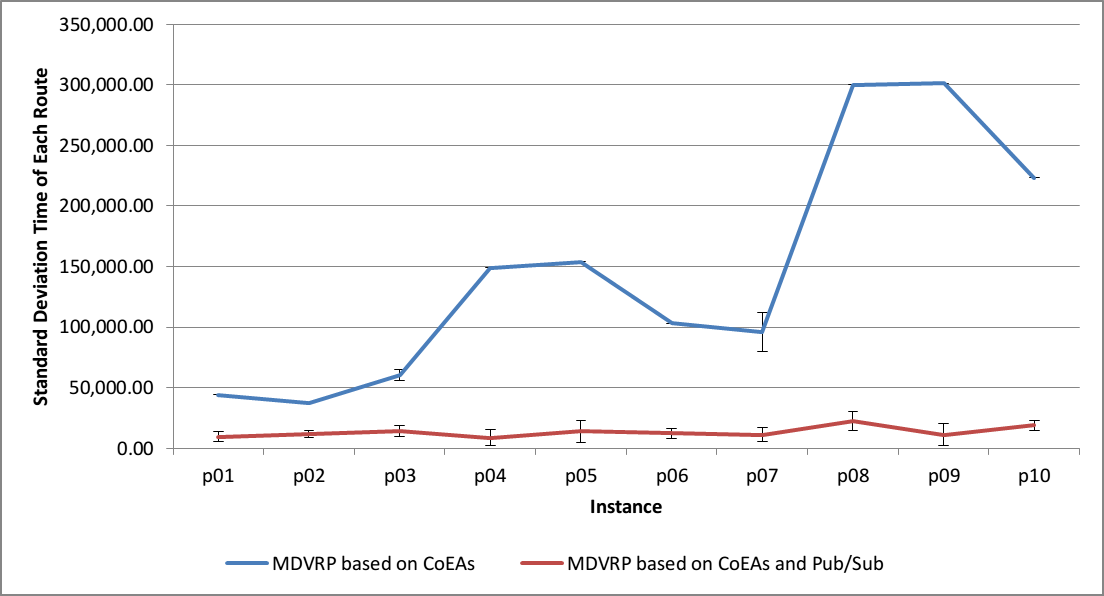
\includegraphics[width=\textwidth]{Resources/Images/test_result_10_cordeau_tw_standard_deviation}
	\caption{Rata-rata standar deviasi total waktu waktu setiap rute dari 5 kali pengujian dengan \textit{service time} pada data Cordeau}
	\label{fig:test_result_10_cordeau_tw_standard_deviation}
\end{figure}


Sementara itu, pada pengujian dengan menggunakan data lapangan, diperoleh hasil sebagaimana digambarkan pada \hyperref[ch:test_result_real_tw]{Lampiran 3}. Kemudian dari seluruh rute yang diperoleh, dikalkulasi waktu total untuk tiap-tiap rute, waktu total dari seluruh rute pada sebuah \textit{instance}, dan standar deviasi total waktu dari masing-masing rute, sebagaimana cara yang dijelaskan pada \autoref{sssec:metric}. 


Berdasarkan \autoref{fig:test_result_4_real_tw_total_time}, diperoleh hasil bahwasannya \textbf{total waktu} yang dihasilkan dengan menggunakan sistem usulan keseluruhannya lebih besar dibandingkan dengan menggunakan aplikasi pembanding, seperti dirincikan pada \autoref{fig:test_result_4_real_tw_total_time}. Sementara dari sisi \textbf{standar deviasi}, keseluruhan \textit{instance} menghasilkan standar deviasi yang lebih kecil, seperti digambarkan pada \autoref{fig:test_result_4_real_tw_standard_deviation}. Hal ini kembali membuktikan efisiensi sistem usulan dibandingkan sistem pembanding karena beban tugas yang lebih merata antar petugas menyebabkan total waktu seluruh kegiatan menjadi lebih pendek.


\begin{longtable}[!]{c|rrrr}
	\caption{Perbandingan total waktu seluruh rute dari pengujian dengan \textit{service time} pada data lapangan TW01 (detik)}
	\label{tbl:test_result_tw01_tw_total_time}\\
	\toprule
	\textit{Pengujian ke} & \MyHead{4cm}{MDVRP berbasis CoEAs} & \MyHead{4cm}{MDVRP berbasis CoEAs dan Pub/Sub} \\ 
	\midrule
	\endfirsthead
	\toprule
	\textit{Pengujian ke} & \MyHead{4cm}{MDVRP berbasis CoEAs} & \MyHead{4cm}{MDVRP berbasis CoEAs dan Pub/Sub} \\ 
	\midrule
	\endhead
	\bottomrule
	\endfoot
	1 & 3.119.907,52 & 3.574.996,52 \\
	2  & 3.121.448,52 & 3.535.812,52 \\
	3  & 3.120.602,52 & 3.457.853,52 \\
	4  & 3.120.658,52 & 3.613.511,52 \\
	5  & 3.120.658,52 & 3.278.235,52 \\
\end{longtable}


\begin{longtable}[!]{c|rrrr}
	\caption{Perbandingan total waktu seluruh rute dari pengujian dengan \textit{service time} pada data lapangan TW02 (detik)}
	\label{tbl:test_result_tw02_tw_total_time}\\
	\toprule
	\textit{Pengujian ke} & \MyHead{4cm}{MDVRP berbasis CoEAs} & \MyHead{4cm}{MDVRP berbasis CoEAs dan Pub/Sub} \\ 
	\midrule
	\endfirsthead
	\toprule
	\textit{Pengujian ke} & \MyHead{4cm}{MDVRP berbasis CoEAs} & \MyHead{4cm}{MDVRP berbasis CoEAs dan Pub/Sub} \\ 
	\midrule
	\endhead
	\bottomrule
	\endfoot
	1 & 7.892.350,51 & 8.136.451,51 \\
	2  & 7.891.082,51 & 8.081.349,51 \\
	3  & 7.892.026,51 & 8.063.507,51 \\
	4  & 7.891.987,51 & 8.084.255,51 \\
	5  & 7.890.758,51 & 8.049.818,51 \\
\end{longtable}


\begin{longtable}[!]{c|rrrr}
	\caption{Perbandingan total waktu seluruh rute dari pengujian dengan \textit{service time} pada data lapangan TW03 (detik)}
	\label{tbl:test_result_tw03_tw_total_time}\\
	\toprule
	\textit{Pengujian ke} & \MyHead{4cm}{MDVRP berbasis CoEAs} & \MyHead{4cm}{MDVRP berbasis CoEAs dan Pub/Sub} \\ 
	\midrule
	\endfirsthead
	\toprule
	\textit{Pengujian ke} & \MyHead{4cm}{MDVRP berbasis CoEAs} & \MyHead{4cm}{MDVRP berbasis CoEAs dan Pub/Sub} \\ 
	\midrule
	\endhead
	\bottomrule
	\endfoot
	1 & 3.166.715,70 & 3.346.362,70 \\
	2  & 3.165.810,70 & 3.301.684,70 \\
	3  & 3.165.810,70 & 3.637.807,70 \\
	4  & 3.166.339,70 & 3.433.349,70 \\
	5  & 3.165.810,70 & 3.337.273,70 \\
\end{longtable}


\begin{longtable}[!]{c|rrrr}
	\caption{Perbandingan total waktu seluruh rute dari pengujian dengan \textit{service time} pada data lapangan TW04 (detik)}
	\label{tbl:test_result_tw04_tw_total_time}\\
	\toprule
	\textit{Pengujian ke} & \MyHead{4cm}{MDVRP berbasis CoEAs} & \MyHead{4cm}{MDVRP berbasis CoEAs dan Pub/Sub} \\ 
	\midrule
	\endfirsthead
	\toprule
	\textit{Pengujian ke} & \MyHead{4cm}{MDVRP berbasis CoEAs} & \MyHead{4cm}{MDVRP berbasis CoEAs dan Pub/Sub} \\ 
	\midrule
	\endhead
	\bottomrule
	\endfoot
	1 & 7.868.523,23 & 8.060.837,23 \\
	2  & 7.867.638,23 & 8.249.584,23 \\
	3  & 7.868.582,23 & 8.081.128,23 \\
	4  & 7.868.543,23 & 7.994.925,23 \\
	5  & 7.866.618,23 & 8.075.293,23 \\
\end{longtable}


\begin{longtable}[!]{c|rrrr}
	\caption{Rata-rata total waktu seluruh rute dari 5 kali pengujian dengan \textit{service time} pada data lapangan (detik)}
	\label{tbl:test_result_real_tw_total_time}\\
	\toprule
	\textit{\textit{Instance}} & \MyHead{4cm}{MDVRP berbasis CoEAs} & \MyHead{4cm}{MDVRP berbasis CoEAs dan Pub/Sub} \\ 
	\midrule
	\endfirsthead
	\toprule
	\textit{\textit{Instance}} & \MyHead{4cm}{MDVRP berbasis CoEAs} & \MyHead{4cm}{MDVRP berbasis CoEAs dan Pub/Sub} \\ 
	\midrule
	\endhead
	\bottomrule
	\endfoot
	tw01 & \textbf{3.120.655,12} & 3.492.081,92 \\
	tw02  & \textbf{7.891.641,11} & 8.083.076,51 \\
	tw03  & \textbf{3.166.097,50} & 3.411.295,70 \\
	tw04  & \textbf{7.867.981,03} & 8.092.353,63 \\
\end{longtable}


\begin{figure}[!]
	\centering
	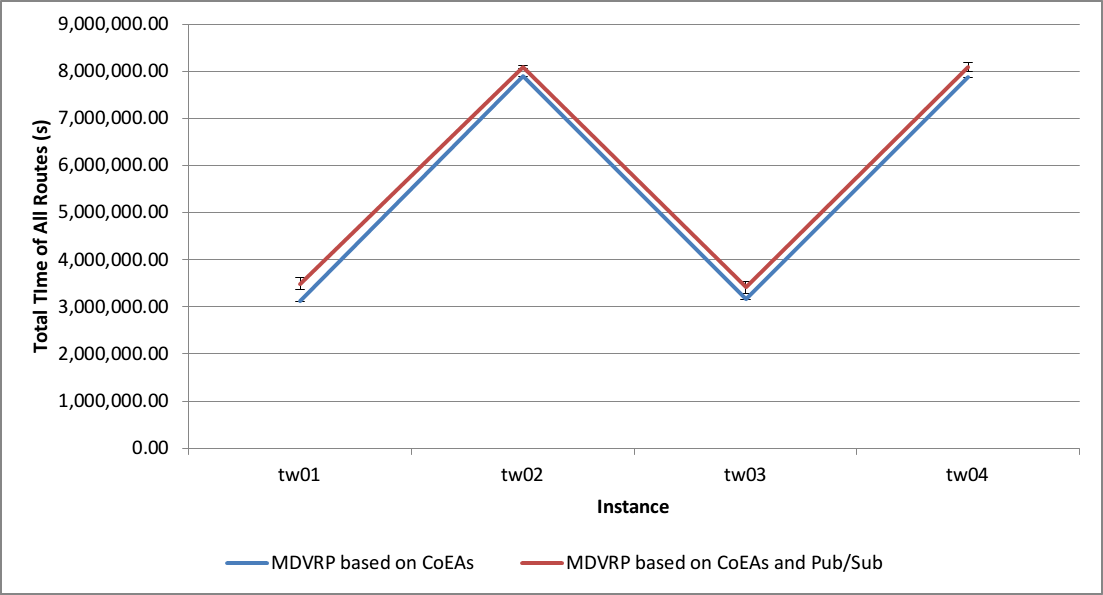
\includegraphics[width=\textwidth]{Resources/Images/test_result_4_real_tw_total_time}
	\caption{Rata-rata total waktu seluruh rute dari 5 kali pengujian dengan \textit{service time} pada data lapangan}
	\label{fig:test_result_4_real_tw_total_time}
\end{figure}


\begin{longtable}[!]{c|rrrr}
	\caption{Perbandingan standar deviasi total waktu setiap rute dari pengujian dengan \textit{service time} pada data lapangan TW01 (detik)}
	\label{tbl:test_result_tw01_tw_standard_deviation_of_total_time}\\
	\toprule
	\textit{Pengujian ke} & \MyHead{4cm}{MDVRP berbasis CoEAs} & \MyHead{4cm}{MDVRP berbasis CoEAs dan Pub/Sub} \\ 
	\midrule
	\endfirsthead
	\toprule
	\textit{Pengujian ke} & \MyHead{4cm}{MDVRP berbasis CoEAs} & \MyHead{4cm}{MDVRP berbasis CoEAs dan Pub/Sub} \\ 
	\midrule
	\endhead
	\bottomrule
	\endfoot
	1 & 82.529,44 & 24.134,25 \\
	2  & 79.711,49 & 21.938,51 \\
	3  & 79.675,78 & 12.895,10 \\
	4  & 82.499,26 & 15.934,00 \\
	5  & 82.499,26 & 16.284,84 \\
\end{longtable}


\begin{longtable}[!]{c|rrrr}
	\caption{Perbandingan standar deviasi total waktu setiap rute dari pengujian dengan \textit{service time} pada data lapangan TW02 (detik)}
	\label{tbl:test_result_tw02_tw_standard_deviation_of_total_time}\\
	\toprule
	\textit{Pengujian ke} & \MyHead{4cm}{MDVRP berbasis CoEAs} & \MyHead{4cm}{MDVRP berbasis CoEAs dan Pub/Sub} \\ 
	\midrule
	\endfirsthead
	\toprule
	\textit{Pengujian ke} & \MyHead{4cm}{MDVRP berbasis CoEAs} & \MyHead{4cm}{MDVRP berbasis CoEAs dan Pub/Sub} \\ 
	\midrule
	\endhead
	\bottomrule
	\endfoot
	1 & 210.200,68 & 17.801,33 \\
	2  & 210.148,28 & 23.662,35 \\
	3  & 202.438,14 & 18.914,64 \\
	4  & 210.223,53 & 27.334,36 \\
	5  & 202.378,65 & 15.324,55 \\
\end{longtable}


\begin{longtable}[!]{c|rrrr}
	\caption{Perbandingan standar deviasi total waktu setiap rute dari pengujian dengan \textit{service time} pada data lapangan TW03 (detik)}
	\label{tbl:test_result_tw03_tw_standard_deviation_of_total_time}\\
	\toprule
	\textit{Pengujian ke} & \MyHead{4cm}{MDVRP berbasis CoEAs} & \MyHead{4cm}{MDVRP berbasis CoEAs dan Pub/Sub} \\ 
	\midrule
	\endfirsthead
	\toprule
	\textit{Pengujian ke} & \MyHead{4cm}{MDVRP berbasis CoEAs} & \MyHead{4cm}{MDVRP berbasis CoEAs dan Pub/Sub} \\ 
	\midrule
	\endhead
	\bottomrule
	\endfoot
	1 & 83.961,70 & 22.296,01 \\
	2  & 83.893,25 & 11.336,41 \\
	3  & 83.893,25 & 22.964,47 \\
	4  & 83.901,64 & 17.708,11 \\
	5  & 83.893,25 & 18.897,75 \\
\end{longtable}


\begin{longtable}[!]{c|rrrr}
	\caption{Perbandingan standar deviasi total waktu setiap rute dari pengujian dengan \textit{service time} pada data lapangan TW04 (detik)}
	\label{tbl:test_result_tw04_tw_standard_deviation_of_total_time}\\
	\toprule
	\textit{Pengujian ke} & \MyHead{4cm}{MDVRP berbasis CoEAs} & \MyHead{4cm}{MDVRP berbasis CoEAs dan Pub/Sub} \\ 
	\midrule
	\endfirsthead
	\toprule
	\textit{Pengujian ke} & \MyHead{4cm}{MDVRP berbasis CoEAs} & \MyHead{4cm}{MDVRP berbasis CoEAs dan Pub/Sub} \\ 
	\midrule
	\endhead
	\bottomrule
	\endfoot
	1 & 205.597,64 & 25.430,96 \\
	2  & 205.550,73 & 26.065,70 \\
	3  & 200.082,02 & 28.568,05 \\
	4  & 205.618,16 & 21.826,97 \\
	5  & 200.067,68 & 30.166,66 \\
\end{longtable}


\begin{longtable}[!]{c|rrrr}
	\caption{Rata-rata standar deviasi total waktu setiap rute dari pengujian dengan \textit{service time} pada data lapangan (detik)}
	\label{tbl:test_result_real_tw_standard_deviation_of_total_time}\\
	\toprule
	\textit{\textit{Instance}} & \MyHead{4cm}{MDVRP berbasis CoEAs} & \MyHead{4cm}{MDVRP berbasis CoEAs dan Pub/Sub} \\ 
	\midrule
	\endfirsthead
	\toprule
	\textit{\textit{Instance}} & \MyHead{4cm}{MDVRP berbasis CoEAs} & \MyHead{4cm}{MDVRP berbasis CoEAs dan Pub/Sub} \\ 
	\midrule
	\endhead
	\bottomrule
	\endfoot
	tw01 & 81.383,05  & \textbf{18.237,34} \\
	tw02  & 207.077,86 & \textbf{20.607,45} \\
	tw03  & 83.908,62  & \textbf{18.640,55} \\
	tw04  & 203.383,25 & \textbf{26.411,67} \\
\end{longtable}


\begin{figure}[!]
	\centering
	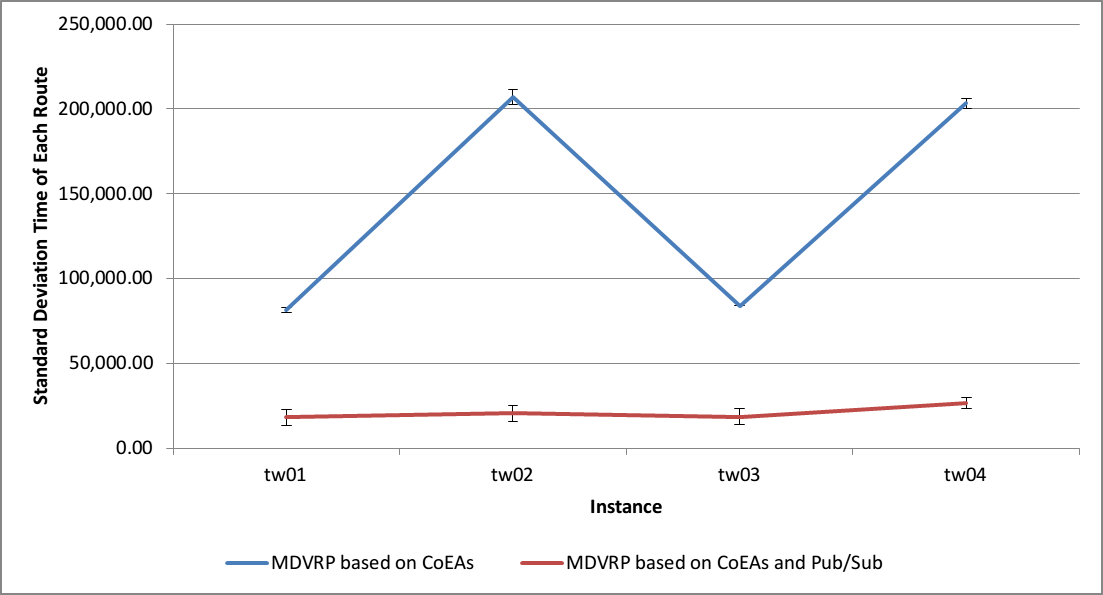
\includegraphics[width=\textwidth]{Resources/Images/test_result_4_real_tw_standard_deviation}
	\caption{Rata-rata standar deviasi total waktu waktu setiap rute dari 5 kali pengujian dengan \textit{service time} pada data lapangan}
	\label{fig:test_result_4_real_tw_standard_deviation}
\end{figure}


%-----------------------------------------------------------------------------%
\subsubsection{Pengujian Kondisi \textit{Delay} dengan \textit{Service Time}}
\label{sssec:test-delay-service-time}
%-----------------------------------------------------------------------------%
Skenario pengujian kondisi \textit{delay} dimaksudkan untuk membandingkan program yang dijalankan pada kondisi terjadi hal-hal yang menghambat jalannya pencacahan. Pengujian ini digunakan sebagai cerminan kodisi lapangan dimana pada beberapa lokasi tidak terdapat koneksi yang stabil, sehingga untuk melakukan \textit{subscription} lokasi berikutnya perlu berpindah ke lokasi lain. Pengujian dilakukan sebanyak 7 (tujuh) kali, dimana tiap-tiap mencerminkan kondisi yang berbeda, yaitu:

\begin{enumerate}
	\item Pengujian dengan kode \textit{instance} d01 menggambarkan kondisi normal. Parameter yang digunakan pada \textit{instance} ini adalah sebagai berikut:
	\begin{itemize}
		\item Jumlah responden pada setiap segmen/blok sensus adalah 10 rumah tangga
		\item Rata-rata wawancara pada setiap rumah tangga 27,58 menit dengan standar deviasi 12,13 menit.
		\item Rata-rata waktu yang diperlukan untuk mendapatkan koneksi internet sebesar 5 menit dengan standar deviasi 3 menit.
	\end{itemize}
	\item Pengujian dengan kode \textit{instance} d02 menggambarkan kondisi dimana anggota rumah tangga sedikit dan relatif homogen, dengan koneksi internet relatif mudah didapatkan. Parameter yang digunakan pada \textit{instance} ini adalah sebagai berikut:
	\begin{itemize}
		\item Jumlah responden pada setiap segmen/blok sensus adalah 10 rumah tangga
		\item Rata-rata wawancara pada setiap rumah tangga 27,58 menit dengan standar deviasi 4,16 menit.
		\item Rata-rata waktu yang diperlukan untuk mendapatkan koneksi internet sebesar 5 menit dengan standar deviasi 3 menit.
	\end{itemize}
	\item Pengujian dengan kode \textit{instance} d03 menggambarkan kondisi dimana anggota rumah tangga sedikit dan relatif homogen, dengan koneksi internet secara umum sulit didapatkan. Parameter yang digunakan pada \textit{instance} ini adalah sebagai berikut:
	\begin{itemize}
		\item Jumlah responden pada setiap segmen/blok sensus adalah 10 rumah tangga
		\item Rata-rata wawancara pada setiap rumah tangga 27,58 menit dengan standar deviasi 4,16 menit.
		\item Rata-rata waktu yang diperlukan untuk mendapatkan koneksi internet sebesar 60 menit dengan standar deviasi 3 menit.
	\end{itemize}
	\item Pengujian dengan kode \textit{instance} d04 menggambarkan kondisi dimana anggota rumah tangga banyak dan relatif homogen, dengan koneksi internet relatif mudah didapatkan. Parameter yang digunakan pada \textit{instance} ini adalah sebagai berikut:
	\begin{itemize}
		\item Jumlah responden pada setiap segmen/blok sensus adalah 10 rumah tangga
		\item Rata-rata wawancara pada setiap rumah tangga 71,58 menit dengan standar deviasi 12,16 menit.
		\item Rata-rata waktu yang diperlukan untuk mendapatkan koneksi internet sebesar 5 menit dengan standar deviasi 3 menit.
	\end{itemize}
	\item Pengujian dengan kode \textit{instance} d05 menggambarkan kondisi dimana anggota rumah tangga banyak dan relatif homogen, dengan koneksi internet secara umum sulit didapatkan. Parameter yang digunakan pada \textit{instance} ini adalah sebagai berikut:
	\begin{itemize}
		\item Jumlah responden pada setiap segmen/blok sensus adalah 10 rumah tangga
		\item Rata-rata wawancara pada setiap rumah tangga 71,58 menit dengan standar deviasi 12,16 menit.
		\item Rata-rata waktu yang diperlukan untuk mendapatkan koneksi internet sebesar 60 menit dengan standar deviasi 3 menit.
	\end{itemize}
	\item Pengujian dengan kode \textit{instance} d06 menggambarkan kondisi dimana rata-rata anggota rumah tangga sedikit tetapi memiliki variasi tinggi, dengan koneksi internet secara umum sulit didapatkan. Parameter yang digunakan pada \textit{instance} ini adalah sebagai berikut:
	\begin{itemize}
		\item Jumlah responden pada setiap segmen/blok sensus adalah 10 rumah tangga
		\item Rata-rata wawancara pada setiap rumah tangga 27,58 menit dengan standar deviasi 25,16 menit.
		\item Rata-rata waktu yang diperlukan untuk mendapatkan koneksi internet sebesar 60 menit dengan standar deviasi 3 menit.
	\end{itemize}
	\item Pengujian dengan kode \textit{instance} d07 menggambarkan kondisi dimana jarak antar rumah tangga jauh, rata-rata anggota rumah tangga banyak dan memiliki variasi tinggi, dan koneksi internet secara umum sulit didapatkan. Parameter yang digunakan pada \textit{instance} ini adalah sebagai berikut:
	\begin{itemize}
		\item Jumlah responden pada setiap segmen/blok sensus adalah 10 rumah tangga
		\item Rata-rata wawancara pada setiap rumah tangga 71,58 menit dengan standar deviasi 25,65 menit.
		\item Rata-rata waktu tempuh antar rumah tangga 30,45 menit dengan standar deviasi 22,12 menit.
		\item Rata-rata waktu yang diperlukan untuk mendapatkan koneksi internet sebesar 60 menit dengan standar deviasi 3 menit.
	\end{itemize}
\end{enumerate}


Dari hasil simulasi, diperoleh rute untuk tiap-tiap \textit{instance} sebagaimana digambarkan pada \hyperref[ch:test_result_delay]{Lampiran 4}. Hasil pengujian seperti digambarkan pada \autoref{fig:test_result_delay_total_time} dan \autoref{fig:test_result_delay_standard_deviation}, dimana masing-masing menunjukkan perbandingan rata-rata waktu total keseluruhan rute dan standar deviasi waktu total dari masing-masing rute, menunjukkan hasil yang relatif sama dan sekaligus menegaskan kembali kesimpulan yang telah diperoleh pada skenario pengujian sebelumnya, yakni sistem usulan lebih efisien dibandingkan sistem pembanding.


\begin{longtable}[!]{c|rrrr}
	\caption{Perbandingan total waktu seluruh rute dari pengujian kondisi \textit{delay} dengan \textit{service time} pada data lapangan D01 (detik)}
	\label{tbl:test_result_d01_tw_total_time}\\
	\toprule
	\textit{Pengujian ke} & \MyHead{4cm}{MDVRP berbasis CoEAs} & \MyHead{4cm}{MDVRP berbasis CoEAs dan Pub/Sub} \\ 
	\midrule
	\endfirsthead
	\toprule
	\textit{Pengujian ke} & \MyHead{4cm}{MDVRP berbasis CoEAs} & \MyHead{4cm}{MDVRP berbasis CoEAs dan Pub/Sub} \\ 
	\midrule
	\endhead
	\bottomrule
	\endfoot
	1 & 3.126.361,44 & 3.532.199,80 \\
	2  & 3.127.305,44 & 3.511.954,08 \\
	3  & 3.127.266,44 & 3.496.727,37 \\
	4  & 3.126.685,44 & 3.326.428,87 \\
	5  & 3.127.629,44 & 3.343.240,98 \\
\end{longtable}


\begin{longtable}[!]{c|rrrr}
	\caption{Perbandingan total waktu seluruh rute dari pengujian kondisi \textit{delay} dengan \textit{service time} pada data lapangan D02 (detik)}
	\label{tbl:test_result_d02_tw_total_time}\\
	\toprule
	\textit{Pengujian ke} & \MyHead{4cm}{MDVRP berbasis CoEAs} & \MyHead{4cm}{MDVRP berbasis CoEAs dan Pub/Sub} \\ 
	\midrule
	\endfirsthead
	\toprule
	\textit{Pengujian ke} & \MyHead{4cm}{MDVRP berbasis CoEAs} & \MyHead{4cm}{MDVRP berbasis CoEAs dan Pub/Sub} \\ 
	\midrule
	\endhead
	\bottomrule
	\endfoot
	1 & 3.107.775,85 & 3.743.549,71 \\
	2  & 3.107.775,85 & 3.570.769,45 \\
	3  & 3.107.775,85 & 3.643.231,06 \\
	4  & 3.107.775,85 & 3.614.051,85 \\
	5  & 3.108.680,85 & 3.543.857,39 \\
\end{longtable}


\begin{longtable}[!]{c|rrrr}
	\caption{Perbandingan total waktu seluruh rute dari pengujian kondisi \textit{delay} dengan \textit{service time} pada data lapangan D03 (detik)}
	\label{tbl:test_result_d03_tw_total_time}\\
	\toprule
	\textit{Pengujian ke} & \MyHead{4cm}{MDVRP berbasis CoEAs} & \MyHead{4cm}{MDVRP berbasis CoEAs dan Pub/Sub} \\ 
	\midrule
	\endfirsthead
	\toprule
	\textit{Pengujian ke} & \MyHead{4cm}{MDVRP berbasis CoEAs} & \MyHead{4cm}{MDVRP berbasis CoEAs dan Pub/Sub} \\ 
	\midrule
	\endhead
	\bottomrule
	\endfoot
	1 & 3.085.573,84 & 3.901.417,79 \\
	2  & 3.087.695,84 & 4.081.770,38 \\
	3  & 3.086.466,84 & 3.888.955,97 \\
	4  & 3.085.297,84 & 4.209.409,21 \\
	5  & 3.086.291,84 & 3.946.962,99 \\
\end{longtable}


\begin{longtable}[!]{c|rrrr}
	\caption{Perbandingan total waktu seluruh rute dari pengujian kondisi \textit{delay} dengan \textit{service time} pada data lapangan D04 (detik)}
	\label{tbl:test_result_d04_tw_total_time}\\
	\toprule
	\textit{Pengujian ke} & \MyHead{4cm}{MDVRP berbasis CoEAs} & \MyHead{4cm}{MDVRP berbasis CoEAs dan Pub/Sub} \\ 
	\midrule
	\endfirsthead
	\toprule
	\textit{Pengujian ke} & \MyHead{4cm}{MDVRP berbasis CoEAs} & \MyHead{4cm}{MDVRP berbasis CoEAs dan Pub/Sub} \\ 
	\midrule
	\endhead
	\bottomrule
	\endfoot
	1 & 7.937.588,57 & 8.262.690,25 \\
	2  & 7.937.642,57 & 8.466.346,59 \\
	3  & 7.938.125,57 & 8.163.875,81 \\
	4  & 7.938.547,57 & 8.249.516,01 \\
	5  & 7.938.586,57 & 8.356.219,55 \\
\end{longtable}


\begin{longtable}[!]{c|rrrr}
	\caption{Perbandingan total waktu seluruh rute dari pengujian kondisi \textit{delay} dengan \textit{service time} pada data lapangan D05 (detik)}
	\label{tbl:test_result_d05_tw_total_time}\\
	\toprule
	\textit{Pengujian ke} & \MyHead{4cm}{MDVRP berbasis CoEAs} & \MyHead{4cm}{MDVRP berbasis CoEAs dan Pub/Sub} \\ 
	\midrule
	\endfirsthead
	\toprule
	\textit{Pengujian ke} & \MyHead{4cm}{MDVRP berbasis CoEAs} & \MyHead{4cm}{MDVRP berbasis CoEAs dan Pub/Sub} \\ 
	\midrule
	\endhead
	\bottomrule
	\endfoot
	1 & 7.903.175,28 & 8.820.620,43 \\
	2  & 7.903.431,28 & 8.884.547,65 \\
	3  & 7.902.425,28 & 8.805.014,14 \\
	4  & 7.901.711,28 & 8.748.018,48 \\
	5  & 7.902.526,28 & 8.928.164,66 \\
\end{longtable}


\begin{longtable}[!]{c|rrrr}
	\caption{Perbandingan total waktu seluruh rute dari pengujian kondisi \textit{delay} dengan \textit{service time} pada data lapangan D06 (detik)}
	\label{tbl:test_result_d06_tw_total_time}\\
	\toprule
	\textit{Pengujian ke} & \MyHead{4cm}{MDVRP berbasis CoEAs} & \MyHead{4cm}{MDVRP berbasis CoEAs dan Pub/Sub} \\ 
	\midrule
	\endfirsthead
	\toprule
	\textit{Pengujian ke} & \MyHead{4cm}{MDVRP berbasis CoEAs} & \MyHead{4cm}{MDVRP berbasis CoEAs dan Pub/Sub} \\ 
	\midrule
	\endhead
	\bottomrule
	\endfoot
	1 & 3.083.461,58 & 4.019.585,94 \\
	2  & 3.082.556,58 & 4.024.606,10 \\
	3  & 3.082.556,58 & 4.225.530,40 \\
	4  & 3.082.514,58 & 4.393.099,78 \\
	5  & 3.083.500,58 & 4.027.765,43 \\
\end{longtable}


\begin{longtable}[!]{c|rrrr}
	\caption{Perbandingan total waktu seluruh rute dari pengujian kondisi \textit{delay} dengan \textit{service time} pada data lapangan D07 (detik)}
	\label{tbl:test_result_d07_tw_total_time}\\
	\toprule
	\textit{Pengujian ke} & \MyHead{4cm}{MDVRP berbasis CoEAs} & \MyHead{4cm}{MDVRP berbasis CoEAs dan Pub/Sub} \\ 
	\midrule
	\endfirsthead
	\toprule
	\textit{Pengujian ke} & \MyHead{4cm}{MDVRP berbasis CoEAs} & \MyHead{4cm}{MDVRP berbasis CoEAs dan Pub/Sub} \\ 
	\midrule
	\endhead
	\bottomrule
	\endfoot
	1 & 10.792.753,12 & 11.590.204,96 \\
	2  & 10.792.792,12 & 11.611.804,84 \\
	3  & 10.792.753,12 & 11.693.081,76 \\
	4  & 10.792.753,12 & 11.615.257,94 \\
	5  & 10.792.214,12 & 11.721.424,91 \\
\end{longtable}


\begin{longtable}[!]{c|rrrr}
	\caption{Rata-rata total waktu seluruh rute dari 5 kali pengujian kondisi \textit{delay} dengan \textit{service time} pada data lapangan (detik)}
	\label{tbl:test_result_delay_tw_total_time}\\
	\toprule
	\textit{\textit{Instance}} & \MyHead{4cm}{MDVRP berbasis CoEAs} & \MyHead{4cm}{MDVRP berbasis CoEAs dan Pub/Sub} \\ 
	\midrule
	\endfirsthead
	\toprule
	\textit{\textit{Instance}} & \MyHead{4cm}{MDVRP berbasis CoEAs} & \MyHead{4cm}{MDVRP berbasis CoEAs dan Pub/Sub} \\ 
	\midrule
	\endhead
	\bottomrule
	\endfoot
	d01 & \textbf{3.127.049,64}  & 3.442.110,22  \\
	d02  & \textbf{3.107.956,85}  & 3.623.091,89  \\
	d03  & \textbf{3.086.265,24}  & 4.005.703,27  \\
	d04  & \textbf{7.938.098,17}  & 8.299.729,64  \\
	d05  & \textbf{7.902.653,88}  & 8.837.273,07  \\
	d06  & \textbf{3.082.917,98}  & 4.138.117,53  \\
	d07  & \textbf{10.792.653,12} & 11.646.354,88 \\
\end{longtable}


\begin{figure}[!]
	\centering
	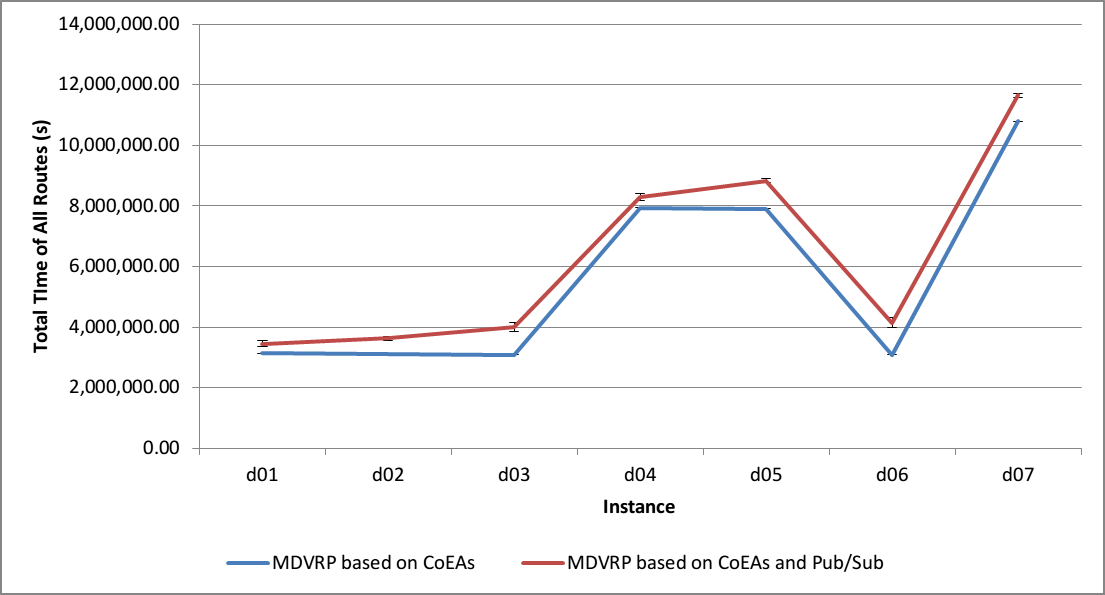
\includegraphics[width=\textwidth]{Resources/Images/test_result_delay_total_time}
	\caption{Rata-rata total waktu seluruh rute dari 5 kali pengujian kondisi \textit{delay} dengan \textit{service time} pada data lapangan}
	\label{fig:test_result_delay_total_time}
\end{figure}


\begin{longtable}[!]{c|rrrr}
	\caption{Perbandingan standar deviasi total waktu setiap rute dari pengujian kondisi \textit{delay} dengan \textit{service time} pada data lapangan D01 (detik)}
	\label{tbl:test_result_d01_tw_standard_deviation_of_total_time}\\
	\toprule
	\textit{Pengujian ke} & \MyHead{4cm}{MDVRP berbasis CoEAs} & \MyHead{4cm}{MDVRP berbasis CoEAs dan Pub/Sub} \\ 
	\midrule
	\endfirsthead
	\toprule
	\textit{Pengujian ke} & \MyHead{4cm}{MDVRP berbasis CoEAs} & \MyHead{4cm}{MDVRP berbasis CoEAs dan Pub/Sub} \\ 
	\midrule
	\endhead
	\bottomrule
	\endfoot
	1 & 85.427,10    & 16.565,69    \\
	2  & 82.688,33    & 14.113,11    \\
	3  & 85.488,25    & 17.278,57    \\
	4  & 82.605,08    & 17.754,52    \\
	5  & 85.461,84    & 16.838,26    \\
\end{longtable}


\begin{longtable}[!]{c|rrrr}
	\caption{Perbandingan standar deviasi total waktu setiap rute dari pengujian kondisi \textit{delay} dengan \textit{service time} pada data lapangan D02 (detik)}
	\label{tbl:test_result_d02_tw_standard_deviation_of_total_time}\\
	\toprule
	\textit{Pengujian ke} & \MyHead{4cm}{MDVRP berbasis CoEAs} & \MyHead{4cm}{MDVRP berbasis CoEAs dan Pub/Sub} \\ 
	\midrule
	\endfirsthead
	\toprule
	\textit{Pengujian ke} & \MyHead{4cm}{MDVRP berbasis CoEAs} & \MyHead{4cm}{MDVRP berbasis CoEAs dan Pub/Sub} \\ 
	\midrule
	\endhead
	\bottomrule
	\endfoot
	1 & 84.873,08    & 13.445,49    \\
	2  & 84.873,08    & 17.693,49    \\
	3  & 84.873,08    & 20.187,86    \\
	4  & 84.873,08    & 18.494,98    \\
	5  & 84.946,37    & 17.371,24    \\
\end{longtable}


\begin{longtable}[!]{c|rrrr}
	\caption{Perbandingan standar deviasi total waktu setiap rute dari pengujian kondisi \textit{delay} dengan \textit{service time} pada data lapangan D03 (detik)}
	\label{tbl:test_result_d03_tw_standard_deviation_of_total_time}\\
	\toprule
	\textit{Pengujian ke} & \MyHead{4cm}{MDVRP berbasis CoEAs} & \MyHead{4cm}{MDVRP berbasis CoEAs dan Pub/Sub} \\ 
	\midrule
	\endfirsthead
	\toprule
	\textit{Pengujian ke} & \MyHead{4cm}{MDVRP berbasis CoEAs} & \MyHead{4cm}{MDVRP berbasis CoEAs dan Pub/Sub} \\ 
	\midrule
	\endhead
	\bottomrule
	\endfoot
	1 & 83.869,48    & 21.175,88    \\
	2  & 83.877,63    & 20.015,83    \\
	3  & 81.057,92    & 19.325,37    \\
	4  & 83.395,96    & 23.602,58    \\
	5  & 81.101,89    & 14.452,49    \\
\end{longtable}


\begin{longtable}[!]{c|rrrr}
	\caption{Perbandingan standar deviasi total waktu setiap rute dari pengujian kondisi \textit{delay} dengan \textit{service time} pada data lapangan D04 (detik)}
	\label{tbl:test_result_d04_tw_standard_deviation_of_total_time}\\
	\toprule
	\textit{Pengujian ke} & \MyHead{4cm}{MDVRP berbasis CoEAs} & \MyHead{4cm}{MDVRP berbasis CoEAs dan Pub/Sub} \\ 
	\midrule
	\endfirsthead
	\toprule
	\textit{Pengujian ke} & \MyHead{4cm}{MDVRP berbasis CoEAs} & \MyHead{4cm}{MDVRP berbasis CoEAs dan Pub/Sub} \\ 
	\midrule
	\endhead
	\bottomrule
	\endfoot
	1 & 204.164,67   & 21.147,45    \\
	2  & 210.888,75   & 23.488,72    \\
	3  & 204.299,39   & 22.320,04    \\
	4  & 210.962,19   & 25.688,13    \\
	5  & 204.198,44   & 19.839,10    \\
\end{longtable}


\begin{longtable}[!]{c|rrrr}
	\caption{Perbandingan standar deviasi total waktu setiap rute dari pengujian kondisi \textit{delay} dengan \textit{service time} pada data lapangan D05 (detik)}
	\label{tbl:test_result_d05_tw_standard_deviation_of_total_time}\\
	\toprule
	\textit{Pengujian ke} & \MyHead{4cm}{MDVRP berbasis CoEAs} & \MyHead{4cm}{MDVRP berbasis CoEAs dan Pub/Sub} \\ 
	\midrule
	\endfirsthead
	\toprule
	\textit{Pengujian ke} & \MyHead{4cm}{MDVRP berbasis CoEAs} & \MyHead{4cm}{MDVRP berbasis CoEAs dan Pub/Sub} \\ 
	\midrule
	\endhead
	\bottomrule
	\endfoot
	1 & 210.500,85   & 26.542,12    \\
	2  & 210.487,04   & 28.747,53    \\
	3  & 202.428,69   & 33.102,26    \\
	4  & 210.496,14   & 17.095,74    \\
	5  & 210.420,26   & 27.118,97    \\
\end{longtable}


\begin{longtable}[!]{c|rrrr}
	\caption{Perbandingan standar deviasi total waktu setiap rute dari pengujian kondisi \textit{delay} dengan \textit{service time} pada data lapangan D06 (detik)}
	\label{tbl:test_result_d06_tw_standard_deviation_of_total_time}\\
	\toprule
	\textit{Pengujian ke} & \MyHead{4cm}{MDVRP berbasis CoEAs} & \MyHead{4cm}{MDVRP berbasis CoEAs dan Pub/Sub} \\ 
	\midrule
	\endfirsthead
	\toprule
	\textit{Pengujian ke} & \MyHead{4cm}{MDVRP berbasis CoEAs} & \MyHead{4cm}{MDVRP berbasis CoEAs dan Pub/Sub} \\ 
	\midrule
	\endhead
	\bottomrule
	\endfoot
	1 & 84.959,86    & 22.071,07    \\
	2  & 84.891,74    & 23.581,69    \\
	3  & 84.891,74    & 12.973,02    \\
	4  & 84.893,54    & 19.175,80    \\
	5  & 82.317,07    & 19.675,74    \\
\end{longtable}

\newpage
\begin{longtable}[!]{c|rrrr}
	\caption{Perbandingan standar deviasi total waktu setiap rute dari pengujian kondisi \textit{delay} dengan \textit{service time} pada data lapangan D07 (detik)}
	\label{tbl:test_result_d07_tw_standard_deviation_of_total_time}\\
	\toprule
	\textit{Pengujian ke} & \MyHead{4cm}{MDVRP berbasis CoEAs} & \MyHead{4cm}{MDVRP berbasis CoEAs dan Pub/Sub} \\ 
	\midrule
	\endfirsthead
	\toprule
	\textit{Pengujian ke} & \MyHead{4cm}{MDVRP berbasis CoEAs} & \MyHead{4cm}{MDVRP berbasis CoEAs dan Pub/Sub} \\ 
	\midrule
	\endhead
	\bottomrule
	\endfoot
	1 & 280.996,99   & 29.048,13    \\
	2  & 270.931,93   & 34.795,38    \\
	3  & 280.996,99   & 29.539,87    \\
	4  & 280.996,99   & 37.706,62    \\
	5  & 280.902,98   & 24.210,62    \\
\end{longtable}


\begin{longtable}[!]{c|rrrr}
	\caption{Rata-rata standar deviasi total waktu setiap rute dari 5 kali pengujian kondisi \textit{delay} dengan \textit{service time} pada data lapangan (detik)}
	\label{tbl:test_result_delay_tw_standard_deviation_of_total_time}\\
	\toprule
	\textit{\textit{Instance}} & \MyHead{4cm}{MDVRP berbasis CoEAs} & \MyHead{4cm}{MDVRP berbasis CoEAs dan Pub/Sub} \\ 
	\midrule
	\endfirsthead
	\toprule
	\textit{\textit{Instance}} & \MyHead{4cm}{MDVRP berbasis CoEAs} & \MyHead{4cm}{MDVRP berbasis CoEAs dan Pub/Sub} \\ 
	\midrule
	\endhead
	\bottomrule
	\endfoot
	d01 & 84.334,12  & \textbf{16.510,03} \\
	d02  & 84.887,74  & \textbf{17.438,61} \\
	d03  & 82.660,58  & \textbf{19.714,43} \\
	d04  & 206.902,69 & \textbf{22.496,69} \\
	d05  & 208.866,60 & \textbf{26.521,32} \\
	d06  & 84.390,79  & \textbf{19.495,46} \\
	d07  & 278.965,18 & \textbf{31.060,12} \\
\end{longtable}


\begin{figure}[!]
	\centering
	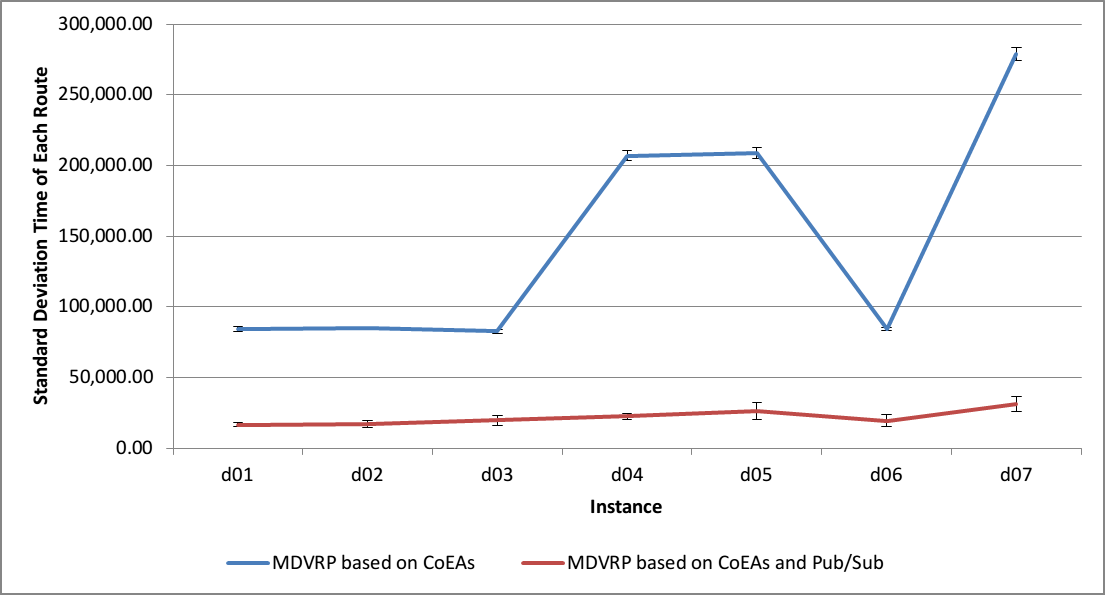
\includegraphics[width=\textwidth]{Resources/Images/test_result_delay_standard_deviation}
	\caption{Rata-rata standar deviasi total waktu setiap rute dari 5 kali pengujian kondisi \textit{delay} dengan \textit{service time} pada data lapangan}
	\label{fig:test_result_delay_standard_deviation}
\end{figure}


%%-----------------------------------------------------------------------------%
%\subsubsection{Pengujian Kondisi Pencacah Berhenti dengan \textit{Service Time}}
%\label{sssec:test-quit-service-time}
%%-----------------------------------------------------------------------------%
%
%
%\begin{longtable}[!]{c|rrrr}
%	\caption{Hasil Pengujian Kondisi Normal Pada Data Cordeau Dengan \textit{Service Time}}
%	\label{tbl:test_result_4_real_tw_delay}\\
%	\toprule
%	\textit{Instance} & \MyHead{2.5cm}{Total Waktu CoES MDVRP (det)} & \MyHead{2.5cm}{Total Waktu CoES MDVRP + Pub/Sub (det)} & \MyHead{2.5cm}{Stdev Waktu CoES MDVRP (det)} & \MyHead{2.5cm}{Stdev Waktu CoES MDVRP + Pub/Sub (det)} \\ 
%	\midrule
%	\endfirsthead
%	\toprule
%	\textit{Instance} & \MyHead{2.5cm}{Total Waktu CoES MDVRP (det)} & \MyHead{2.5cm}{Total Waktu CoES MDVRP + Pub/Sub (det)} & \MyHead{2.5cm}{Stdev Waktu CoES MDVRP (det)} & \MyHead{2.5cm}{Stdev Waktu CoES MDVRP + Pub/Sub (det)} \\ 
%	\midrule
%	\endhead
%	\bottomrule
%	\endfoot
%	q01 &  & 3,464,733.76 &  & 37,997.03 \\
%	q02 &  & 3,635,752.13 &  & 68,239.51 \\
%	q03 &  & 3,611,394.03 &  & 98,900.33 \\
%\end{longtable}



